\documentclass[12pt]{report}

\usepackage{tamuconfig}

% Most of the packages that set the default settings
% for the document have moved to the style file
% tamuconfig.sty.

%These next lines change the font. Fixes for certain
%fonts will be implemented in a future release.

%Comment this line if you do not wish to use Times
%New Roman. The font used will then be the LaTeX
%default of Computer Modern.
\usepackage{times}
%\usepackage{cmbright}
\usepackage[T1]{fontenc}

%This package allows for the use of graphics in the
%document.
\usepackage{amsmath, amsthm, amssymb, amsfonts, booktabs, graphicx, float, esint, subcaption, xspace, xcolor}

%\usepackage{stix}
\usepackage{stmaryrd}
\usepackage{hyperref}

%If you have JPEG format images, add .jpg as an
%allowed file extension below. Same for Bitmaps (.bmp).
\DeclareGraphicsExtensions{.png}

%It is best practice to keep all your pictures in
%one folder inside the main directory in which your
%TeX file is kept. Here the folder is named "graphic."
%Replace the name here with your folder's name, if needed.
%The period is needed due to relative referencing.
\graphicspath{ {./graphic/} }

%%%%%%%%%%%%%%%%%%%%%%%%%%%%%%%%%%%%%%%%%%%%%%%%%%%%%%%%%
%Please place all your personal packages here. Check to
%see if the packages you wish to use are not already
%declared above. Placing all your personal packages
%here allows me to determine if there are any package
%issues in compilation, as well as any conflicts
%that may arise by the order of loading.
%--Sean Zachary Roberson
%%%%%%%%%%%%%%%%%%%%%%%%%%%%%%%%%%%%%%%%%%%%%%%%%%%%%%%%%
%%%%%%%%%%%%%%%%%%%%%%%%%%%%%%%%%%%%%%%%%%%%%%%%%%%%%%%%%
%Begin student defined packages.
%%%%%%%%%%%%%%%%%%%%%%%%%%%%%%%%%%%%%%%%%%%%%%%%%%%%%%%%%


\setlength{\abovedisplayskip}{0pt}
\setlength{\belowdisplayskip}{0pt}
\setlength{\abovedisplayshortskip}{0pt}
\setlength{\belowdisplayshortskip}{0pt}

\newcommand{\vr}{\vec{r}}
\newcommand{\vp}{\vec{p}}
\newcommand{\vOmega}{\vec{\Omega}}
\newcommand{\vJ}{\vec{J}}
\newcommand{\vO}{\vec{\Omega}}
\newcommand{\bra}{\left\langle}
\newcommand{\ket}{\right\rangle}
\newcommand{\braSN}{\left\langle \! \left\langle}
\newcommand{\ketSN}{\right\rangle \! \right\rangle}
\newcommand{\sbraSN}{\left[ \! \left[}
\newcommand{\sketSN}{\right] \! \right]}
\newcommand{\sbra}{\left[}
\newcommand{\sket}{\right]}
\renewcommand{\div}{\vec{\nabla} \cdot}
\newcommand{\grad}{\vec{\nabla}}
\newcommand{\vbeta}{\vec{\beta} }
\newcommand{\pdx}{\frac{\partial}{\partial x}}
\newcommand{\pdy}{\frac{\partial}{\partial y}}
\newcommand{\pdz}{\frac{\partial}{\partial z}}
\newcommand{\intrrr}{\int d^3 r \,}
\newcommand{\intrr}{\int d^2 r \,}
\newcommand{\dEdphi}{\partial_\phi E }
\newcommand{\dEdp}{\partial_p E }
\newcommand{\dBdphi}{\partial_\phi B }
\newcommand{\dBdp}{B }
\newcommand{\adj}{\phi^\dag}
\newcommand{\vefadj}{\varphi^\dag}
\newcommand{\surf}{\int_{\partial V}}
\newcommand{\domain}{V}
\newcommand{\bound}{\partial V}
\newcommand{\vn}{\vec{n}}
\newcommand{\Edd}{\mathbb{E}}
\newcommand{\BEdd}{B}
\newcommand{\sigt}{\sigma_t}
\newcommand{\sigs}{\sigma_s}
\newcommand{\siga}{\sigma_a}
%\newcommand{\isigt}{\sigma_t^{-1}}
%\newcommand{\isigtp}{\sigma_{t,p}^{-1}}
\newcommand{\isigt}{\ell_t}
\newcommand{\isigtp}{\ell_{t,p}}
\newcommand{\angSource}{\frac{q}{4 \pi}}
\newcommand{\angSourcep}{\frac{q_p}{4 \pi}}
\newcommand{\angSourcepd}{\frac{q_p+\delta q_p}{4 \pi}}
\newcommand{\angSourced}{\frac{\delta q_p}{4 \pi}}
\newcommand{\scalSource}{q}
\newcommand{\angResp}{q^\dag}
\newcommand{\scalResp}{q^\dag}
\newcommand{\qoi}{{\it QoI}\xspace}


\newcommand{\comment}[2]{\marginpar{\textcolor{#2}{$\star$}}\textcolor{#2}{#1}\newline}

%-----------------------------------------------------------
%-----------------------------------------------------------
\usepackage{ifthen}
\newboolean{draftversion}
\setboolean{draftversion}{true}
%-----------------------------------------------------------
%----------------------------------------------------------

\ifthenelse{\boolean{draftversion}}
{
\newcommand{\iwh}[1]{\comment{#1}{red}}
\newcommand{\jcr}[1]{\comment{#1}{blue}}
\newcommand{\todo}[1]{\comment{#1}{purple}}
}
{
\newcommand{\iwh}[1]{\phantom{a}}
\newcommand{\jcr}[1]{\phantom{a}}
\newcommand{\todo}[1]{\phantom{a}}
}
\newcommand{\tcr}[1]{\comment{#1}{red}}

%%%%%%%%%%%%%%%%%%%%%%%%%%%%%%%%%%%%%%%%%%%%%%%%%%%%%%%%%
%End student defined packages.
%%%%%%%%%%%%%%%%%%%%%%%%%%%%%%%%%%%%%%%%%%%%%%%%%%%%%%%%%

% End preamble. Document begins below.

\begin{document}

%The title of your document goes here.
%Spacing may need to be adjusted if your title is long
%and pushes the copyright off the page.
\renewcommand{\tamumanuscripttitle}{Adjoint-based sensitivity for radiation transport using an Eddington tensor formulation}

%Type only Thesis, Dissertation, or Record of Study.
\renewcommand{\tamupapertype}{Thesis DRAFT}

%Your full name goes here, as it is in university records. Check your student record on Howdy if there is any mismatch.
\renewcommand{\tamufullname}{Ian Halvic}

%The degree title goes here. See the OGAPS site for more info.
\renewcommand{\tamudegree}{Master of Science}
\renewcommand{\tamuchairone}{Professor Jean Ragusa}


% Uncomment out the next line if you have co-chairs.  You will also need to edit the titlepage.tex file.
%\newcommand{\tamuchairtwo}{Additional Chair Name}
\renewcommand{\tamumemberone}{Professor Marvin Adams}
\newcommand{\tamumembertwo}{Professor Bojan Popov}
\renewcommand{\tamudepthead}{Professor Yassin Hassan}

%Type only May, August, or December.
\renewcommand{\tamugradmonth}{March}
\renewcommand{\tamugradyear}{2018}
%Your department name goes here.
\renewcommand{\tamudepartment}{Nuclear Engineering}


%%%%%%%%%%%%%%%%%%%%%%%%%%%%%%%%%%%%%%%%%%%%%%%%%%%
%
%  New template code for TAMU Theses and Dissertations starting Fall 2016.  
%
%
%  Author: Sean Zachary Roberson
%  Version 3.17.06
%  Last Updated: 6/15/2017
%
%%%%%%%%%%%%%%%%%%%%%%%%%%%%%%%%%%%%%%%%%%%%%%%%%%%

%%%%%%%%%%%%%%%%%%%%%%%%%%%%%% 
%% TITLE PAGE
%% The values get updated automatically.  Please do not make changes to this file other than adding/deleting committee members where necessary.
%%%%%%%%%%%%%%%%%%%%%%%%%%%%%%

\providecommand{\tabularnewline}{\\}



\begin{titlepage}
\begin{center}
\MakeUppercase{\tamumanuscripttitle}
\vspace{4em}

A \tamupapertype

by

\MakeUppercase{\tamufullname}

\vspace{4em}

\begin{singlespace}

Submitted to the Office of Graduate and Professional Studies of \\
Texas A\&M University \\

in partial fulfillment of the requirements for the degree of \\
\end{singlespace}

\MakeUppercase{\tamudegree}
\par\end{center}
\vspace{2em}
\begin{singlespace}
\begin{tabular}{ll}
 & \tabularnewline
& \cr
% If you have Co-Chairs comment out the 'Chair of Committee' line below and uncomment the 'Co-Chairs of Committee' line.
Chair of Committee, & \tamuchairone\tabularnewline
%Co-Chairs of Committee, & \tamuchairone\tabularnewline & \tamuchairtwo\tabularnewline
Committee Members, & \tamumemberone\tabularnewline
 & \tamumembertwo\tabularnewline
% & \tamumemberthree\tabularnewline
Head of Department, & \tamudepthead\tabularnewline

\end{tabular}
\end{singlespace}
\vspace{3em}

\begin{center}
\tamugradmonth \hspace{2pt} \tamugradyear

\vspace{3em}

Major Subject: \tamudepartment \par
\vspace{3em}
Copyright \tamugradyear \hspace{.5em}\tamufullname 
\par\end{center}
\end{titlepage}
\pagebreak{}




 % This is simply a file that formats and adds your titlepage, please do not edit this unless you have a specific need. .
%%%%%%%%%%%%%%%%%%%%%%%%%%%%%%%%%%%%%%%%%%%%%%%%%%%
%%%%%%%%%%%%%%%%%%%%%%%%%%%%%%%%%%%%%%%%%%%%%%%%%%%%%%%%%%%%%%%%%%%%%
%%                           ABSTRACT 
%%%%%%%%%%%%%%%%%%%%%%%%%%%%%%%%%%%%%%%%%%%%%%%%%%%%%%%%%%%%%%%%%%%%%

\chapter*{ABSTRACT}
\addcontentsline{toc}{chapter}{ABSTRACT} % Needs to be set to part, so the TOC doesnt add 'CHAPTER ' prefix in the TOC.

\pagestyle{plain} % No headers, just page numbers
\pagenumbering{roman} % Roman numerals
\setcounter{page}{2}

\todo{I need to loop back to this}
Adjoint methods can provide a first-order approximation of the response a physical system due to a perturbation in the system's parameters. However, when applying the method to a time dependent transport, memory costs can quickly become a concern, and a fully angular dependent flux must be stored at each timestep. Here, a lower-order Variable Eddington Tensor formulation of the transport equation is considered to remove the angular dependence of the stored solution and reduce memory costs. Indeed, given the Eddington tensor, the Eddington tensor approach yields the same answer as the full transport solution.

In the case of perturbations, one may make some simplifying assumption regarding the Eddington tensor: for instance, keep it unperturbed or assuming a functional variation of the Eddington tensor over the input parameter space. An unperturbed Eddington assumption may introduce error in the sensitivity calculation. A simple linear interpolation scheme for the Eddington over the uncertain parameter range is devised for use in certain scenarios, at the cost of requiring a few additional forward Sn-solves to parameterize the Eddington tensor. Results highlighting the approach are presented. An alternate formulation using an Eddington tensor derived from the adjoint transport is also presented, and shows promise in particular scenarios. Comparison of the derived Eddington methods and transport methods is done using slab geometry test cases.


 

\pagebreak{}

%%%%%%%%%%%%%%%%%%%%%%%%%%%%%%%%%%%%%%%%%%%%%%%%%%%%%%%%%%%%%%%%%%%%%%
%%                           DEDICATION
%%%%%%%%%%%%%%%%%%%%%%%%%%%%%%%%%%%%%%%%%%%%%%%%%%%%%%%%%%%%%%%%%%%%%
\chapter*{DEDICATION}
\addcontentsline{toc}{chapter}{DEDICATION}  % Needs to be set to part, so the TOC doesnt add 'CHAPTER ' prefix in the TOC.



\begin{center}
\vspace*{\fill}
\todo{Add Dedications Here}
\vspace*{\fill}
\end{center}

\pagebreak{}

%%%%%%%%%%%%%%%%%%%%%%%%%%%%%%%%%%%%%%%%%%%%%%%%%%%%%%%%%%%%%%%%%%%%%%
%%                           ACKNOWLEDGMENTS
%%%%%%%%%%%%%%%%%%%%%%%%%%%%%%%%%%%%%%%%%%%%%%%%%%%%%%%%%%%%%%%%%%%%%
\chapter*{ACKNOWLEDGMENTS}
\addcontentsline{toc}{chapter}{ACKNOWLEDGMENTS}  % Needs to be set to part, so the TOC doesnt add 'CHAPTER ' prefix in the TOC.
I would like to thank my advisor Professor Jean Ragusa for his invaluable help on this work and other academic endeavors. 



\pagebreak{}
%%%%%%%%%%%%%%%%%%%%%%%%%%%%%%%%%%%%%%%%%%%%%%%%%%%%%%%%%%%%%%%%%%%%%%
%%             CONTRIBUTORS AND FUNDING SOURCES
%%%%%%%%%%%%%%%%%%%%%%%%%%%%%%%%%%%%%%%%%%%%%%%%%%%%%%%%%%%%%%%%%%%%%
\chapter*{CONTRIBUTORS AND FUNDING SOURCES}
\addcontentsline{toc}{chapter}{CONTRIBUTORS AND FUNDING SOURCES}  % Needs to be set to part, so the TOC doesn't add 'CHAPTER ' prefix in the TOC.


%This section is taken directly from the MS Word templates.

%Old version below.

%All theses and dissertations must include a contributors and funding sources section. In this section, name all members of the dissertation committee, and any collaboration with others in carrying out your thesis or dissertation research. Your independent contributions must be made clear.
%
%If financial support from the university or any other source was gained to conduct your thesis or dissertation research and compilation, it must be listed in this section. If you completed all work independently without outside financial support, indicate this here.
%\textit{(Sample Wording)}
%
%This work was supported by a dissertation committee consisting of Professor XXX [advisor – also note if co-advisor] and XXXX of the Department of [Home Department] and Professor(s) XXXX of the Department of [Outside Department].
% 
%The data analyzed for Chapter III was provided by Professor XXXX. The analyses depicted in Chapter IV were conducted in part by Rebecca Jones of the Department of Biostatistics and were published in (year) in an article listed in the Biographical Sketch. 
%
%All other work conducted for the dissertation was completed by the student independently.
%
%\noindent \textit{(or)}
%
%This work was supervised by a dissertation committee consisting of Professor XXXX [advisor – also note if co-advisor] and Professor(s) XXXX of the Department of [Home Department] and Professor(s) XXXX of [Outside Department]. All work for the dissertation was completed independently by the student.
%
%\noindent \textit{(or)}
%
%Graduate study was supported by a fellowship from Texas A\&M University and a dissertation research fellowship from XXX Foundation.

\subsection*{Contributors}
This work was supported by a thesis (or) dissertation committee consisting of Professor Jean Ragusa and Professor Marvin Adams of the Department of Nuclear Engineering and Professor Bojan Popov of the Department of Mathematics.


All other work conducted for the thesis (or) dissertation was completed by the student independently.
\subsection*{Funding Sources}
Graduate study was supported by a fellowship from Texas A\&M University and a dissertation research fellowship from XXX Foundation. 
\pagebreak{}
%%%%%%%%%%%%%%%%%%%%%%%%%%%%%%%%%%%%%%%%%%%%%%%%%%%%%%%%%%%%%%%%%%%%%%
%%                           NOMENCLATURE
%%%%%%%%%%%%%%%%%%%%%%%%%%%%%%%%%%%%%%%%%%%%%%%%%%%%%%%%%%%%%%%%%%%%%

\chapter*{NOMENCLATURE}
\addcontentsline{toc}{chapter}{NOMENCLATURE}  % Needs to be set to part, so the TOC doesnt add 'CHAPTER ' prefix in the TOC.

%A note about aligning: These entries will align
%themselves according to the ampersand (&).
%No extra spaces are needed, as seen in some of
%the entries below.

%Example of the longtable environment.
\hspace*{-1.25in}
\vspace{12pt}
\begin{spacing}{1.0}
	\begin{longtable}[htbp]{@{}p{0.35\textwidth} p{0.62\textwidth}@{}}
	   % \begin{tabular}{@{}p{0.33\textwidth} p{0.62\textwidth}@{}}
		VET 		& Variable Eddington Tensor\\	[2ex]
		aVET 		& Adjoint Variable Eddington Tensor\\	[2ex]
		SN 			& Discrete Ordinate Method\\	[2ex]
	   % \end{tabular}%
	\end{longtable}
\end{spacing}

\pagebreak{}

%%%%%%%%%%%%%%%%%%%%%%%%%%%%%%%%%%%%%%%%%%%%%%%%%%%
%
%  New template code for TAMU Theses and Dissertations starting Fall 2016.  
%
%
%  Author: Sean Zachary Roberson
%  Version 3.17.06
%  Last Updated: 6/15/2017
%
%%%%%%%%%%%%%%%%%%%%%%%%%%%%%%%%%%%%%%%%%%%%%%%%%%%
%%%%%%%%%%%%%%%%%%%%%%%%%%%%%%%%%%%%%%%%%%%%%%%%%%%%%%%%%%%%%%%%%%%%%%
%%       TABLE OF CONTENTS
%%%%%%%%%%%%%%%%%%%%%%%%%%%%%%%%%%%%%%%%%%%%%%%%%%%%%%%%%%%%%%%%%%%%%
% single-space sections in Table of Contents  - commented in version 1.7
%\renewcommand{\cftsecafterpnum}{\vskip0.5\baselineskip}
%\renewcommand{\cftsubsecafterpnum}{\vskip0.5\baselineskip}
%\renewcommand{\cftsubsubsecafterpnum}{\vskip0.5\baselineskip}
%%%%%%%%%%%%%%%%%%%%%%%%%%%%%%%%%%%%%%%%%%%%%%%%%%%

\phantomsection
\addcontentsline{toc}{chapter}{TABLE OF CONTENTS}  

\begin{singlespace}
\renewcommand\contentsname{\normalfont} {\centerline{TABLE OF CONTENTS}}

\setcounter{tocdepth}{4} % This puts \subsubsection[]{×} in your List of Tables.  The default is 3.


%%%%%%%%%%%%%  Adds Page above the page number in TOC
\setlength{\cftaftertoctitleskip}{1em}
\renewcommand{\cftaftertoctitle}{%
\hfill{\normalfont {Page}\par}}


\tableofcontents

%\addtocontents{toc}{\protect\afterpage{~\hfill\normalfont{Page}\par\medskip}}
\end{singlespace}

\pagebreak{}

%%%%%%%%%%%%%%%%%%%%%%%%%%%%%%%%%%%%%%%%%%%%%%%%%%%%%%%%%%%%%%%%%%%%%%
%%                           LIST OF FIGURES
%%%%%%%%%%%%%%%%%%%%%%%%%%%%%%%%%%%%%%%%%%%%%%%%%%%%%%%%%%%%%%%%%%%%%

\phantomsection
\addcontentsline{toc}{chapter}{LIST OF FIGURES}  

\renewcommand{\cftloftitlefont}{\center\normalfont\MakeUppercase}

\setlength{\cftbeforeloftitleskip}{-12pt} %% Positions the LOF title vertically to match the chapter titles
\renewcommand{\cftafterloftitleskip}{12pt}


\renewcommand{\cftafterloftitle}{%
\\[4em]\mbox{}\hspace{2pt}FIGURE\hfill{\normalfont Page}\vskip\baselineskip}

\begingroup


\begin{center}
\begin{singlespace}
%% These values make the lof table entries appear double spaced between.
\setlength{\cftbeforechapskip}{0.4cm}
\setlength{\cftbeforesecskip}{0.30cm}
\setlength{\cftbeforesubsecskip}{0.30cm}
\setlength{\cftbeforefigskip}{0.4cm}
\setlength{\cftbeforetabskip}{0.4cm}

% Provided by Andy Philips.
% needed to make chapter gaps look no different than sections:
% \addtocontents{lof}{\protect\renewcommand*\protect\addvspace[1]{}}

% Philips' document had 30 figures. Is there a maximum number of figures
% that changes the spacing to non-uniform, i.e., not double-spaced
% between all entries?

\listoffigures

\end{singlespace}
\end{center}

\pagebreak{}


%%%%%%%%%%%%%%%%%%%%%%%%%%%%%%%%%%%%%%%%%%%%%%%%%%%%%%%%%%%%%%%%%%%%%%
%%                           LIST OF TABLES
%%%%%%%%%%%%%%%%%%%%%%%%%%%%%%%%%%%%%%%%%%%%%%%%%%%%%%%%%%%%%%%%%%%%%%
%
\phantomsection
\addcontentsline{toc}{chapter}{LIST OF TABLES}  

\renewcommand{\cftlottitlefont}{\center\normalfont\MakeUppercase}

\setlength{\cftbeforelottitleskip}{-12pt} %% Positions the LOT title vertically to match the chapter titles

%Note that the similar parameter in the LOF is 12pt; this
%is intentional to make the spacing between the headers
%and the first entry look consistent.
\renewcommand{\cftafterlottitleskip}{1pt}


\renewcommand{\cftafterlottitle}{%
\\[4em]\mbox{}\hspace{2pt}TABLE\hfill{\normalfont Page}\vskip\baselineskip}

\begin{center}
\begin{singlespace}

%% These values make the lot table entries appear double spaced between.
\setlength{\cftbeforechapskip}{0.4cm}
\setlength{\cftbeforesecskip}{0.30cm}
\setlength{\cftbeforesubsecskip}{0.30cm}
\setlength{\cftbeforefigskip}{0.4cm}
\setlength{\cftbeforetabskip}{0.4cm}

\listoftables 

\end{singlespace}
\end{center}
\endgroup
\pagebreak{}  % Need this for the pagenumbering to be correct.   % This is simply a file that formats and adds your toc, lof, and lot, please do not edit this unless you have a specific need.

%%%%%%%%%%%%%%%%%%%%%%%%%%%%%%%%%%%%%%%%%%%%%%%%%%%%%%%%%%%%%%%%%%%%%%
%%                           SECTION I
%%%%%%%%%%%%%%%%%%%%%%%%%%%%%%%%%%%%%%%%%%%%%%%%%%%%%%%%%%%%%%%%%%%%%


\pagestyle{plain} % No headers, just page numbers
\pagenumbering{arabic} % Arabic numerals
\setcounter{page}{1}


\chapter{\uppercase {Introduction}}

%%%%%%%%%%%%%%%%%%%%%%%%%%%%%%%%%%%%%%%%%%%%%%%%%%%%%%%%%%%%%%%%%%%%%%%%%%%%%%%%%%%%%%%%%%%%%%%%%%%%
\section{Introduction}
%%%%%%%%%%%%%%%%%%%%%%%%%%%%%%%%%%%%%%%%%%%%%%%%%%%%%%%%%%%%%%%%%%%%%%%%%%%%%%%%%%%%%%%%%%%%%%%%%%%%

Computational simulations have become important tools for engineers and scientists across a wide array of disciplines. These simulations allow for researchers to examine significantly complex and long life systems in a way that is frequently more economical in both time and money than construction of the real world system, if even feasible. An important step in creating one of these methods is confirmation that the results can be trusted to reasonably approximate the real life scenario. This can be accomplished using three processes outlined by the National Research Council \cite{NRCVVUQ}


\begin{itemize}
\item Verification - How accurately does the computation solve the underlying equations of the model for the quantities of interest?
\item Validation - How accurately does the model represent reality for the quantities of interest?
\item Uncertainty Quantification (UQ) -  How do the various sources of error and uncertainty feed into uncertainty in the model-based prediction of the quantity of interest?
\end{itemize}


Adjoint methods are particularly useful for UQ. In general, adjoint methods provide a mechanism for computing quantities
 of interest (\qoi) and sensitivity coefficients and, more generally, for propagating uncertainty in the 
 system variables to the error in the desired quantity of interest. They accomplish this in a particularly economical 
 way, requiring only two full system solves (one forward and one adjoint solve) in steady state in order to determine 
 first-order sensitivity coefficients for any combination of sources of uncertainty, as opposed to performing multiple 
 forward system solves to determine the sensitivity due to each individual uncertain parameter.

Using operator notation to denote the forward and adjoint (linear\footnote{The forward problem may be nonlinear, i.e., 
using $\mathbf{A}(u)$, but the adjoint problem is linear, evaluated at $u$ if the forward problem is nonlinear, i.e., 
using $\mathbf{A}^\dag(u)$}) problems, $\mathbf{A}u=q$ and $\mathbf{A}^\dag u^\dag = q^\dag$, respectively, and the 
bracket notation for inner products over the phase space, it is easy to note that a \qoi can be
obtained using {\it either} the forward solution $u$ folded with the response function of interest 
(which is also the adjoint source, $q^\dag$) {\it or} the adjoint solution folded with the forward source~:
\[
\qoi := \bra u, q^\dag \ket = \bra u, \mathbf{A}^\dag u^\dag \ket = 
\bra \mathbf{A} u , u^\dag \ket = \bra q, u^\dag\ket \,.
\]
The sensitivity coefficient due to parameter $p$ can be obtained using two forward solves
\[
\delta_p \qoi = \frac{\qoi^\prime - \qoi}{\delta p} = \frac{ \bra (u^\prime - u), q^\dag \ket}{p^\prime - p}  \,,
\]
where the superscript $^\prime$ denotes a perturbed value. However, one may employ the unperturbed adjoint solution to obtain
a {\it first-order} estimate of the sensitivity coefficient
\[
\delta_p \qoi = \bra u^\dag, \delta_p q - \delta_p \mathbf{A} u \ket  + \mathcal{O}(\delta^2)\,.
\]
The subsequent sections will provide derivations and additional details and will apply these formulations to neutron transport problems. However, it is already evident that if the forward source $q$ is uncertain and only a few \qoi are requested (i.e., only a few response functions $q^\dag$ are needed), then it is preferable to employ the adjoint formulation to compute the quantity of interest (one needs only one adjoint solution per response function $q^\dag$). Furthermore, the first-order sensitivity of the
\qoi to many uncertain parameters is more advantageously computed using the adjoint formalism.

\jcr{I did already point out that this was a repeat. Can you deal with this, blend what needs to be blended in and remove the rest. If this is where you mention previous work related to using an adjoint approach, the literature review needs to be seriously beefed-up. 2-3 citations are not a lot for a thesis. It seems that most of the UQ adjoint literature review happens in the introduction, so augment this. you are mentioning time-dependent problems and the need to save the adjoint at various times (checkpointing), there are clever algo for that too, reference them...}
Adjoint methods are of particular interest for UQ. In general, adjoint methods provide a mechanism for propagating uncertainty and error in the system variables to the error in the desired quantity of interest. Adjoint methods accomplish this in a particularly economical way, sometimes requiring only two differential system solves which can then be used for any combination of sources of error, as opposed to performing an independent solve for each individual error scenario. These adjoint methods have been applied across various complex and time dependent systems. An example of adjoint methods applied to hydrodynamic systems with shocks can be found in Wildey et al. \cite{Wildey}. A more relevant adjoint example to neutron transport occurs in Stripling et al. in the form of reactor burn-up equations \cite{Stripling}.


Application of the adjoint method to time-dependent transport can pose a major technical limitation. In general, the adjoint method applied to radiation transport requires storing six-dimensional data (the forward angular flux) at each time step. When dealing with high resolution in these six dimensions and many time steps, this can potentially require an unreasonable amount of memory for data storage, rendering the method functionally unusable. For the previously mentioned depletion reactor problem of Stripling, this limitation was not existent because a quasi-static approximation was used for the neutron transport equation and only isotopic concentrations were time-dependent. For time-independent radiation problems, only storing the converged scattering moments at defined checkpoints (in burnup) is sufficient to reconstruct the flux solution. If a flux solution is requested outside of the checkpointed burnups, the forward flux can be reconstructed by interpolation \cite{Stripling}.
Using converged scattering source term, a single transport sweep is needed to recover the converged
angular flux. However this method does not extend to time-dependent transport in general because
the primary time-dependent variable, the angular flux, needs to be stored as well. 

A potential solution to the memory requirement for the time-dependent transport adjoint formulation is the use of a quasi-diffusion method to reduce the overall dimensionality of the transport problem, from 6D+time (space, direction, energy, time for transport) to 4D+time (space, energy, time for quasi-diffusion). The method examined in this work is termed  as a ``Variable Eddington Tensor'' formulation and uses the unperturbed forward angular flux to compute the Eddington tensor needed in the quasi-diffusion approach.


\jcr{at some point, you need to say: This Thesis is organized as follows: in Chapter xx, we discuss blabla. ...... FORESHADOW}

%%%%%%%%%%%%%%%%%%%%%%%%%%%%%%%%%%%%%%%%%%%%%%%%%%%%%%%%%%%%%%%%%%%%%%%%%%%%%%%%%%%%%%%%%%%
\chapter{\uppercase {Background (Transport)}}
%%%%%%%%%%%%%%%%%%%%%%%%%%%%%%%%%%%%%%%%%%%%%%%%%%%%%%%%%%%%%%%%%%%%%%%%%%%%%%%%%%%%%%%%%%%%%%%%%%%%
\jcr{foreshadow: what is this chapter about? what will you discuss in the various sections ...?}
%%%%%%%----------------------------------------------------------------------------------------------
\section{Steady-state One-group Neutron Transport Equation}
%%%%%%%----------------------------------------------------------------------------------------------
\jcr{the first sentences actually need to go before the section. according to the section's title, this should be about the SS 1-g transport, not why you are looking at that model. that must come before. I am adding new lines to make it obvious where the break needs to be.}
\jcr{is this the first time you use the term quasi-diffusion? if so, it clearly needs to be defined before, maybe in the introduction chapter}
This work will focus on a relatively simple transport equation form, the one-group steady-state transport equation. Examination of effectiveness of an adjoint formalism using the quasi-diffusion approximation instead of the full transport solution in this setting will provide insight to the advantages and shortcomings of the technique when applied to multigroup, time-dependent transport equation. \jcr{you must mention that the appendix xyz contains a derivation of the time-dependent version approach where we think VET could be useful}


The one-group steady-state transport equation with isotropic sources and isotropic scattering for a volume $V$ bounded by its surface $\partial V$ is given below.
\begin{equation}
\label{SS1GTE}
\vO \cdot \grad \psi(\vr,\vO) + \sigt(\vr) \psi(\vr,\vO) = \frac{1}{4 \pi} \sigs(\vr) \phi(\vr) + \frac{1}{4 \pi} q(\vr), \quad \forall \vr \in V
\end{equation}
\begin{equation}
\label{SS1GTE_bc}
\psi(\vr,\vO) = \psi^{\text{inc}}(\vr,\vO) \quad \vr \in \partial V^{-} = \{ \vr \in \partial V, \text{ s.t. }, \vO \cdot \vec{n}(\vr) < 0\}
\end{equation}
The possibly uncertain parameters in this system are: the total and scattering cross sections $\sigt$ and $\sigs$, the volumetric source term $q$, and the incident angular flux on the system given by $\psi^{\text{inc}}$. The unknowns (dependent variables) are the angular flux $\psi(\vr,\vO)$ and the scalar flux $\phi(\vr)$ given by
\[
\phi(\vr) = \int_{4\pi}d\Omega\,\psi(\vr,\vO) \,.
\]
%%%%%%%----------------------------------------------------------------------------------------------
%\subsection{Quantity of interest and their sensitivities}
%%%%%%%----------------------------------------------------------------------------------------------

%----------------------------------------------------------------------------------------------
\subsection{Quantity of Interest, Response Functions, and Inner Products}
%----------------------------------------------------------------------------------------------
Frequently, the solution to the transport equation is not the sought after value, but rather some Quantity of Interest (\qoi), a functional that depends on the transport solution. Given $\psi(\vr,\vO)$, the solution of the one-group steady-state transport (Eq.~\eqref{SS1GTE}), and $R(\vr, \vO)$, a ``response function'' specific to the desired \qoi, the quantity of interest is defined as
\begin{equation}
\qoi =  \int_V dV \int_{4 \pi} d \vO \,  R(\vr, \vO) \psi(\vr, \vO)
\end{equation}
The response function $R$ can take on physically defined forms, such as the cross section of a detector; or it may take a form of a mathematical construct, such as $R(\vr, \vO)=1/v$ to return the total number of neutrons present in the system. Another example is to let $R(\vr, \vO)=\sigma \chi(\vr)$ to obtain the total \tcr{reactor} in a portion of the domain ($\chi(\vr)=1$ if $\vr \in$ region of interest, and 0 otherwise). Note that the response function will frequently be expressed as $q^\dag$, the adjoint source, as we have already noted that there is a relationship between the solution, the adjoint solution, and their respective source terms. 

Two volumetric inner products are defined using  the $\braSN \bullet , \bullet \ketSN$ and $\bra \bullet , \bullet \ket$ notations. These two inner-products are for use with angular and scalar fluxes, respectively. 
\begin{subequations}
\begin{equation}
\braSN \psi , f \ketSN  = \int_V dV \int_{4 \pi} d \Omega \,  \psi(\vr, \vO)f(\vr, \vO) \,,
\end{equation}
\begin{equation}
\bra \phi(\vr) , f \ket  = \int_V dV \,  \phi(\vr) g(\vr) \,.
\end{equation}
\end{subequations}
For later use, two additional inner products are also defined as surface integrals over the domain 
boundary $\partial V$. The second definition is used to distinguish between incoming and outgoing surface integrals.
\begin{subequations}
\begin{equation}
\sbraSN \psi , g \sketSN  = \int_{\bound} dS \int_{4 \pi} d \Omega \, \vO \cdot \vn(\vr) \, \psi(\vr, \vO)g(\vr, \vO) \,,
\end{equation}
\begin{equation}
\sbraSN \psi , g \sketSN_{\pm}   = \int_{\bound} dS \int_{\vO \cdot \vn \gtrless 0} d\Omega \,  \vO \cdot \vn(\vr) \, \psi(\vr, \vO)g(\vr, \vO) \,.
\end{equation}
\end{subequations}
Therefore, with this notation, the quantity of interest can be compactly expressed as shown below.
\begin{equation}
\label{QoIDef}
\qoi = \braSN \psi(\vr,\vO), \scalResp(\vr) \ketSN  = \bra \phi(\vr) , \scalResp(\vr) \ket
\end{equation}

%----------------------------------------------------------------------------------------------
\subsection{Sensitivity Coefficients}
%----------------------------------------------------------------------------------------------
A hurdle in utilizing the transport equation numerically to make real world predictions is that 
the system's parameters ($\sigt$, $\sigs$, $q$, and $\psi^{inc}$) may not be known exactly. This uncertainty in 
the system parameters is expected to translate to an uncertainty in the \qoi value. Ideally, a reasonable error 
range would be determined for each system parameter and the system simulation would run over a finely 
discretized parameter space, using the resulting \qoi values to generate an error range for the \qoi. 
However, this straightforward method tends to be resource-intensive, requiring a complete forward solve 
of the transport equation for each input uncertainty scenario. Adjoint methods offer a way to drastically 
reduce the number of solves, while generally remaining fairly accurate for small perturbations around 
base or nominal values of the parameters.

%%%%%%%----------------------------------------------------------------------------------------------
\section{Adjoint Sensitivity}
%%%%%%%----------------------------------------------------------------------------------------------

Adjoint operators can provide a useful tool for sensitivity calculations. Using inner product 
notation consider the system of interest $\mathbf{A} \psi = q$. Call this this 
the forward system, with forward operator $\mathbf{A}$. Consider a test function $\psi^\dag$, the 
adjoint operator $\mathbf{A^\dag}$ is defined such that $\braSN \mathbf{A} \psi, \psi^\dag \ketSN = \braSN \psi, 
\mathbf{A^\dag} \psi^\dag \ketSN $. For differential operators, derivation of $\mathbf{A^\dag}$ generally relies on 
application of the divergence theorem (integration by parts), typically resulting in boundary 
terms ($BC$). Using the response function of the desired \qoi, the adjoint system can be constructed 
as $\mathbf{A^\dag} \psi^\dag = q^\dag$, leading to an alternate expression of the \qoi using the 
adjoint solution $\psi^\dag $.
\begin{equation}
\label{genAdjQoI}
\qoi = \braSN \psi, \scalResp \ketSN = \braSN q , \psi^\dag \ketSN + BC
\end{equation} 
From the above \jcr{what? where? there was no actual rigorous derivation above}, it follows that a first-order approximation to the change in the quantity of interest ($\delta \qoi$)
based on perturbations to the initial system, including perturbation to the forward 
operator $\delta \mathbf{A}$ and forward source $\delta q$, can be expressed in the inner product form shown in Eq.~\eqref{genAdjSens} \cite{Marchuk}. Derivation of this begins with the perturbed system $\mathbf{A}_p \psi_p = q_p$ multiplied by the adjoint function $\psi^\dag$ defined above. After expressing the perturbations in a $\delta$ form a first order approximation of $\delta \mathbf{A} \delta \psi = 0$ is used. An integration by parts is used to transpose $\mathbf{A}$ to $\mathbf{A^\dag}$, resulting in boundary terms appearing. 
\begin{equation}
\begin{split}
\braSN \mathbf{A}_p \psi_p ,\psi^\dag\ketSN &= \braSN q_p ,\psi^\dag \ketSN \\
\braSN \left( \mathbf{A}+\delta \mathbf{A} \right) \left( \psi + \delta \psi \right),\psi^\dag\ketSN &= \braSN q+\delta q ,\psi^\dag \ketSN \\
\braSN \mathbf{A} \psi +\delta \mathbf{A} \psi + \mathbf{A} \delta \psi ,\psi^\dag\ketSN &\approx \braSN q+\delta q ,\psi^\dag \ketSN \\
\braSN \mathbf{A} \psi + \mathbf{A} \delta \psi ,\psi^\dag\ketSN &= \braSN q+\delta q - \delta \mathbf{A} \psi  ,\psi^\dag \ketSN \\
\braSN \psi +\delta \psi , \mathbf{A^\dag} \psi^\dag\ketSN &= \braSN q+\delta q - \delta \mathbf{A} \psi  ,\psi^\dag \ketSN + BC \\
\braSN \psi_p , q^\dag \ketSN &= \braSN q+\delta q - \delta \mathbf{A} \psi  ,\psi^\dag \ketSN + BC \\
\end{split}
\end{equation}
The left side of the final step of the above derivation is the perturbed \qoi. Subtracting Eq.~\eqref{genAdjQoI} from this yields the desired expression for the $\delta\qoi$.
\begin{equation}
\label{genAdjSens}
\delta \qoi \approx \braSN \delta q - \delta \mathbf{A} \psi , \psi^\dag \ketSN + \delta BC
\end{equation}
The advantage of the above expression for $\delta\qoi$ is that two solves, one for the forward and another for the adjoint, can be used to approximate the sensitivity for a variety of operator and source perturbations, $\delta \mathbf{A}$ and $\delta q$.

%%%%%%%----------------------------------------------------------------------------------------------
\subsection{Adjoint Formulation for Transport}
%%%%%%%----------------------------------------------------------------------------------------------
In a fairly straightforward application of the adjoint method previously shown, 
\begin{equation}
\label{SnAdjDeriv}
\begin{split}
\braSN \frac{q}{4 \pi} , \psi^\dag  \ketSN  
=& \braSN \vO \cdot \grad \psi + \sigt \psi - \frac{\sigs}{4 \pi} \phi, \psi^\dag \ketSN \\
=& \braSN \vO \cdot \grad \psi, \psi^\dag \ketSN  + \braSN \sigt \psi, \psi^\dag \ketSN  - \braSN \frac{\sigs}{4 \pi}  \phi, \psi^\dag \ketSN \\
=& - \braSN  \psi, \vO \cdot \grad \psi^\dag \ketSN  + \braSN \psi, \sigt \psi^\dag \ketSN  - \braSN   \psi, \frac{\sigs}{4 \pi} \phi^\dag \ketSN + \sbraSN \psi^\dag,  \psi \sketSN\\
=& \braSN  \psi,-  \vO \cdot \grad \psi^\dag  +  \sigt \psi^\dag -  \frac{\sigs}{4 \pi} \phi^\dag \ketSN + \sbraSN \psi^\dag,  \psi \sketSN\\
=& \braSN  \psi,q^\dag \ketSN + \sbraSN \psi^\dag,  \psi \sketSN\\
\end{split}
\end{equation}
the adjoint equation which corresponds to the transport formulation with adjoint source (response function)
$\angResp$ is

\begin{subequations}
\begin{equation}
\label{anAdj}
- \vO \cdot \grad \psi^\dag + \sigt \psi^\dag = \frac{\sigs}{4 \pi} \phi^\dag + \scalResp
\end{equation}
\begin{equation}
\psi^\dag(\vr) = \psi^{\dag, \text{out}}(\vr)=0 \quad \vr \in \partial V^{+} = \{  \vr \in \bound , \quad \vO \cdot \vec{n} > 0 \}
\end{equation}
\end{subequations}
where the definition of the adjoint scalar flux $\phi^\dag$ is analogous to that of 
the forward scalar flux. It is worth noting that the adjoint equation is in the form of the standard transport equation, only with the direction of travel reversed ($\vO \to -\vO)$. This often allows for forward SN transport solvers to be easily adapted to solving the SN adjoint system. Once the adjoint solution is obtained, the corresponding \qoi can be calculated with a simple inner product with the forward source term, as follows from equations Eq.~\eqref{genAdjQoI} and Eq.~\eqref{SnAdjDeriv}. 
\begin{equation}
\label{snAdjQoI}
\qoi := \braSN  \psi,q^\dag \ketSN = \braSN \psi^\dag , \angSource \ketSN - \sbraSN \psi^\dag,  \psi \sketSN
\end{equation}
%
The surface interval in \eqref{snAdjQoI} can be split into incoming and outgoing flux integrals, 
\[
\sbraSN \psi^\dag, \psi \sketSN_- 
= \sbraSN \psi^\dag,  \psi^{\text{inc}} \sketSN_- + \sbraSN \psi^{\dag,\text{out}},\psi \sketSN_+
\]
which are handled by the forward and adjoint boundary conditions respectively. Setting $\psi^{\dag, \text{out}}=0$ removes the outgoing flux integral:
%
\begin{equation}
\label{snAdjQoIBCsplit}
\begin{split}
\qoi &= \braSN \psi^\dag , \angSource \ketSN - \sbraSN \psi^\dag,  \psi^{\text{inc}} \sketSN_- \\
&= \bra \phi^\dag , \angSource \ket - \sbraSN \psi^\dag,  \psi^{\text{inc}} \sketSN_- \,.
\end{split}
\end{equation}

\jcr{in the thesis, remember to explain that the adjoint source is not to be divided by 2 even when the response is isotropic in angle}
\todo{Go into detail about which source to use, angular vs scalar source. Looking forward, I think this has an impact when considering the different adjoint forms: VET of the adjoint vs adjoint of the VET.}
%%%%%%%----------------------------------------------------------------------------------------------
\subsection{Transport Adjoint Sensitivity}
%%%%%%%----------------------------------------------------------------------------------------------

Now consider perturbations to our system. Specifically perturbations of $\delta \sigt$, $\delta \sigs$, and $\delta q$ to the total cross section, scattering cross section and angular source term respectively. In addition, the incident angular flux is also perturbed by $\delta \psi^{inc}$. These perturbations result in a perturbed solution to the SN-transport equation $\psi_p$. 
\begin{equation}
\label{snFwdPert}
\vO \cdot \grad \psi_p + \sigma_{t,p} \psi_p = \frac{\sigma_{s,p}}{4 \pi} \phi_p + \frac{q_p}{4\pi},  \quad \forall \vr \in V
\end{equation}
\begin{equation}
\psi_p(\vr) = \psi_p^{\text{inc}}(\vr), \quad \forall \vr \in \partial V^{-}
\end{equation}
Any quantity with a subscript $p$ is to be understood as the perturbed value, that is, as 
the sum of the unperturbed value and the perturbation amount: $a_p = a + \delta a$.

This perturbation may result in a change to the \qoi, now given by $\qoi_p=\bra \psi_p , \angResp \ket$. Note that we assumed that the response function (adjoint source) was not affected by the perturbation. Using the {\it unperturbed} adjoint equation given in Eq.~\eqref{snAdj},
the perturbed \qoi can be expressed as:
\begin{equation}
\label{snSensPart}
\begin{split}
QoI_p &=\braSN \psi_p , \angResp \ketSN \\
&=\braSN \psi_p , - \vO \cdot \grad \psi^\dag + \sigt \psi^\dag - \frac{\sigs}{4 \pi} \phi^\dag  \ketSN \\
\end{split}
\end{equation}
Next, we perform an integration by parts and obtain:
\begin{equation}
\label{snSensPart2}
QoI_p = \braSN  \vO \cdot \grad \psi_p + \sigt \psi_p - \frac{\sigs}{4 \pi} \phi_p , \psi^\dag  \ketSN - \sbraSN \psi_p, \psi^\dag \sketSN
\end{equation}
Note that the cross sections are unperturbed in Eq.~\eqref{snSensPart2}.
Using a $\delta$ notation for the perturbed system variables ($\sigma_{s,p} = \sigs + \delta \sigs$ for example), we
can introduce the perturbed quantities:
\begin{equation}
\label{snSensPart3}
\begin{split}
QoI_p &= \braSN  \vO \cdot \grad \psi_p + (\sigma_{t,p}- \delta\sigt)\psi_p - \frac{\sigma_{s,p}-\delta \sigs}{4 \pi} \phi_p
 , \psi^\dag  \ketSN - \sbraSN \psi_p, \psi^\dag \sketSN \\
 &= \braSN  \angSourcep - \delta\sigt\psi_p + \frac{\delta \sigs}{4 \pi} \phi_p
 , \psi^\dag  \ketSN - \sbraSN \psi_p, \psi^\dag \sketSN
\end{split}
\end{equation}
Next, note that the cross section terms have double perturbations terms $\delta \sigt \delta \psi$ and $\delta \sigs \delta \psi$ once it is observed
that $\psi_p=\psi+\delta\psi$. In a first-order approximation, these doubly perturbed terms are ignored, yielding:
\begin{equation}
\label{snAdjQoIp}
QoI_p \approx \braSN  \frac{q+\delta q}{4\pi} - \delta\sigt\psi + \frac{\delta \sigs}{4 \pi} \phi
 , \psi^\dag  \ketSN - \sbraSN \psi_p, \psi^\dag \sketSN \,.
\end{equation}

Subtraction of the unperturbed \qoi expression in Eq.~\eqref{snAdjQoI} supplies a final equation for computing the change in \qoi using only the system perturbations and the unperturbed forward solution $\psi$ and the adjoint unperturbed
solution $\psi^\dag$, removing the need to solve the perturbed forward equation. 
Furthermore the boundary terms can be split into incoming and outgoing contributions.
Using a zero outgoing boundary condition for the adjoint flux
(thus $\sbra \delta \psi, \psi^{\dag,\text{out}} \sket_+=0$), one obtains the final 
form of the perturbation in the \qoi.
\begin{equation}
\label{snSens}
\begin{split}
\delta QoI &= \braSN \frac{\delta q}{4\pi} - \delta \sigt \psi + \frac{\delta\sigs}{4 \pi} \phi  , \psi^\dag  \ketSN - \sbraSN \delta \psi, \psi^\dag \sketSN \\
&= \braSN \angSourced - \delta \sigt \psi + \frac{\delta\sigs}{4 \pi} \phi , \psi^\dag  \ketSN - \sbraSN \delta \psi^{\text{inc}}, \psi^\dag \sketSN_- \\
&= \bra \angSourced  + \frac{\delta\sigs}{4 \pi} \phi , \phi^\dag  \ket - \braSN  \delta \sigt \psi , \psi^\dag \ketSN - \sbraSN \delta \psi^{\text{inc}}, \psi^\dag \sketSN_- \,.
\end{split}
\end{equation}
Note that in the final formula, only the forward and adjoint scalar fluxes
are required to evaluate the first-order sensitivity due to perturbations in either the isotropic external source or the isotropic scattering source term. However, the flux angular fluxes are needed to evaluation sensitivities due to
perturbations int he total cross section. Finally, the angular fluxes
are also needed to assess sensitivity due to the boundary source, but these inner
products concern only the domain boundary and the memory storage requirements for these are small compared to volumetric inner products.

%%%%%%%%%%%%%%%%%%%%%%%%%%%%%%%%%%%%%%%%%%%%%%%%%%%%%%%%%%%%%%%%%%%%%%%%%%%%%%%%%%%%%%%%%%%
\chapter{\uppercase {Variable Eddington Tensor Formulations For Adjoint-based Uncertainty Quantification}}
%%%%%%%%%%%%%%%%%%%%%%%%%%%%%%%%%%%%%%%%%%%%%%%%%%%%%%%%%%%%%%%%%%%%%%%%%%%%%%%%%%%%%%%%%%%%%%%%%%%%

%%%%%%%%%%%%%%%%%%%%%%%%%%%%%%%%%%%%%%%%%%%%%%%%%%%%%%%%%%%%%%%%%%%%%%%%%%%%%%%%%%%%%%%%%%%%%%%%%%%%
\section{Motivation for Sensitivity Analysis based on Variable Eddington Tensor Formulations}
%%%%%%%%%%%%%%%%%%%%%%%%%%%%%%%%%%%%%%%%%%%%%%%%%%%%%%%%%%%%%%%%%%%%%%%%%%%%%%%%%%%%%%%%%%%%%%%%%%%%

%%%%%%%----------------------------------------------------------------------------------------------
%\subsection{Motivation} 
%%%%%%%----------------------------------------------------------------------------------------------
While the adjoint transport sensitivity formulation given by Eq.~\eqref{snSens} provides a first-order accurate method to determine the sensitivity to multiple perturbation scenarios using only one forward transport solve and one adjoint transport solve, it can quickly run into limitations for time-dependent systems, where the forward and adjoint systems in space, energy, and angle must be stored at various time moments for subsequent retrieval to compute the sensitivities $\delta \qoi$. For a 3-d geometry, this translates to storing the angular
flux data across 6-dimensions (space/energy/angle). For time independent systems, Stripling \cite{Stripling} showed that a converged scattering source can be stored to reconstruct 
the forward steady-state transport solution on the fly. For time-dependent problems, one possibility to circumvent the storage issues is to employ a Variable Eddington Tensor (VET) approach (which only requires
storing a space/energy, hence 4-d, solution at various moments in time), provided that input parameter perturbations do not affect the values of the Eddington tensor. In this work,
we investigate this question in the simpler setting a steady-state simulations.
\jcr{in the MS thesis, expand on how this would work for time-dependent problems. the entire
gist of the VET idea was to simplify sensitivity calculations for TD transport, so you need
to demonstrate/explain that the ideas you applied in SS were actually going to be useful as well for TD}

\todo{Add in more detail about time dependence. The ideal scenario would be to add in the Eddington equation with time derivatives, however that wouldn't make sense at this exact point in the thesis, as we haven't even derived the steady-state Eddington formulation yet. After a qualitative discussion here, consider looping back towards the end of thesis, presenting the time-dependent VET formulation.}

\iwh{Going to place the derivation in an appendix. This is requested in a few places, not sure if you want it both here and earlier.}

%%%%%%%----------------------------------------------------------------------------------------------
\subsection{Forward VET Formulation}
%%%%%%%----------------------------------------------------------------------------------------------

A VET formulation will reduce the memory requirements when using the adjoint method for sensitivity evaluations. To present the VET formulation, the zero-th and first angular moments of steady-state transport equation are computed by application of the $\int d \Omega$ and $\int d \Omega \, \vO$ operators to Eq.~\eqref{1gTE}, respectively. Using the notation

\begin{equation}
\label{VETFormStart}
\phi(\vr)=\int d\Omega \, \psi( \vr,\vO )
,\quad
\vec{J}(\vr)= \int d\Omega \, \vO \psi( \vr,\vO ) \,,
\end{equation}
the zero-th and first angular moment transport equations are~: 
%
\begin{subequations}
%
\begin{equation}
\label{0am}
\div \vec{J} + (\sigt-\sigs) \phi = \scalSource \,,
\end{equation}
and
\begin{equation}
\label{1am}
\div \left(  \int d\Omega \vO \vO \psi \right) + \sigt \vec{J} = 0 \,.
\end{equation}
%
\end{subequations}
The Eddington Tensor $\Edd$ is then introduced to relate the second angular moment term in equation \eqref{1am} to the scalar flux. The caveat to the Eddington Tensor is that it requires the angular flux solution be known.
\begin{equation}
\label{EddDef}
\Edd(\vr)=\frac{\int d\Omega \vO \vO \psi(\vr,\vO)}{\phi(\vr)} \,.
\end{equation}Note that the Eddington tensor is spatially dependent.
The inclusion of the Eddington tensor allows Eq.~\eqref{1am} to be expressed as 
\begin{equation}
\label{currentE}
\vec{J} = - \frac{1}{\sigt} \div \Edd \phi \,.
\end{equation}
If $\psi(\vr,\vO)$ is a linear function in angle, then $\Edd(\vr)=\tfrac{1}{3}\mathbb{I}$ and one recovers Fick's law for the neutron diffusion current, $\vec{J} = - \frac{1}{3\sigt} \grad \phi$ (note the change from $\div$ to $\grad$). Using Eq.~\eqref{currentE} for the definition of $\vec{J}$ allows us to convert Eq.~\eqref{0am} to the form shown in \eqref{VEFForm}, which only has the scalar flux as an unknown. The substitution $\siga = \sigt-\sigs$ was also used.
\begin{equation}
\label{VEFForm}
- \div \left( \frac{1}{\sigt}\div \Edd \phi \right) + \siga \phi = \scalSource \,.
\end{equation}
The known incident angular flux can be used to generate a suitable boundary conditions using a 
``Boundary Eddington Factor'' $\BEdd(\vr)$ \cite{Miften}. Multiplying the transport boundary condition,
Eq.~\eqref{SS1GTE_bc}, by $2 | \vO \cdot \vn |$, we obtain, for $\vr \in \bound$,
\begin{equation}
2 J^{\text{inc}}(\vr) \equiv  2 \int_{\vO \cdot \vn <0 }  d \Omega\, | \vO \cdot \vec{n} | \psi^{\text{inc}}(\vr,\vO) 
= 2\int_{\vO \cdot \vn <0 } d \Omega\,  | \vO \cdot \vn |  \psi(\vr,\vO) \,.
\end{equation}
$J^{\text{inc}}$ is the partial incoming current. 
Manipulating the second half-range integral yields:
\begin{equation}
2 J^{\text{inc}}(\vr) = \int_{4\pi} d \Omega\,  \left( | \vO \cdot \vn |- \vO\cdot\vn\right)  \psi(\vr,\vO) 
= \BEdd(\vr) \phi(\vr) - \vn(\vr) \cdot \vJ(\vr)
\end{equation}
with $\vJ$ the net current. The boundary Eddington factor is defined as
\begin{equation}
\BEdd(\vr) = \frac{\int_{4 \pi} d\Omega \, | \vO \cdot \vn | \psi}{\int_{4\pi} d\Omega \, \psi} ,\ \ \vr \in \bound \,.
\end{equation}
$\vJ$ can substituted using \eqref{currentE} to get the final form of the VET forward boundary condition:
\begin{equation}
2 J^{\text{inc}} = \BEdd \phi + \vn \cdot \frac{1}{\sigt} \div \Edd \phi \,.
\end{equation}
Note that the Robin boundary conditions for diffusion is recovered when $\Edd = \tfrac{1}{3} \mathbb{I}$ and $B=\tfrac{1}{2}$:
\[
2 J^{\text{inc}} = \frac{\phi}{2} + \vn \cdot \frac{1}{3\sigt} \grad \phi \,.
\]


%%%%%%%----------------------------------------------------------------------------------------------
\subsection{Adjoint VET Formulation}
%%%%%%%----------------------------------------------------------------------------------------------
\jcr{here, adding the graph you used in the presentation could be useful to give the larger picture of the approach you are about to explain}


Since the VET formulation generates a new forward equation to describe the system, a new adjoint corresponding to Eq.~\eqref{VEFForm} must also be formulated. The typical adjoint process is followed in which the forward equation is multiplied by a test function and all operators are transferred to the test function using integration by parts. The following notation is used: $(\grad \grad u)_{ij} = \partial_{x_i} \partial_{x_j} u$
and a tensor dot product $\mathbb{A} : \mathbb{B} = \sum_i \sum_j A_{ij}B_{ij}$.
Next, we compute $\bra \scalSource , \vefadj \ket$ and use the forward VET balance equation, Eq.~\eqref{VEFForm}:
\begin{equation}
\label{VEFadjFormDeriv}
\begin{split}
\bra \scalSource , \vefadj \ket &= - \bra \div \left( \frac{1}{\sigt}\div \Edd \phi \right), \vefadj \ket +  \bra \siga \phi, \vefadj \ket   \\
&= \bra \frac{1}{\sigt}\div \Edd \phi, \grad \vefadj \ket  +  \bra  \phi, \siga \vefadj \ket - \sbra \vn \cdot \frac{1}{\sigt}\div \Edd \phi, \vefadj \sket   \\
 &=  - \bra \phi, \Edd : \left( \grad \left( \frac{1}{\sigt}\grad \vefadj \right) \right) \ket  +  \bra  \phi, \siga \vefadj \ket \\
 &\quad\quad  - \sbra \vn \cdot  \frac{1}{\sigt}\div \Edd \phi, \vefadj \sket + \sbra \phi, \vn \cdot  \Edd \cdot \frac{1}{\sigt} \grad \vefadj \sket  \,,
\end{split}
\end{equation}
where the new boundary inner product for use with VET is defined as
\begin{equation}
\sbra \phi(\vr) , g(\vr)  \sket = \int_{\partial V} dS \, \phi (\vr) g (\vr)  \,.
\end{equation}
Note that we used the fact that the Eddington tensor is symmetric, $\Edd^T=\Edd$.
\jcr{can you verified on the side, say for 2d $xy$ that the integration by parts does yield the boundary terms. I am worried about the successive $\cdot$'s.}
This leads to the adjoint equation of the VET formulation, given in Eq.~\eqref{adjForm}. Of particular note is that the double divergence term present in the forward equation contributes to a double gradient term in the adjoint equation below. The VET adjoint solution is represented by $\vefadj$ to avoid confusion with $\phi^\dag$, which is the adjoint scalar flux from the SN transport  method. 

\begin{equation}
\label{adjForm}
- \Edd : \left( \grad \left( \frac{1}{\sigt}\grad \vefadj \right) \right) + \siga \vefadj = \scalResp
\end{equation}
By inspection of the boundary terms in Eq.~\eqref{VEFadjFormDeriv} and for reasons that will become apparent during sensitivity calculations, the boundary condition chosen for the adjoint equation is given in Eq.~\eqref{adjVETBC}.
\begin{equation}
\label{adjVETBC}
2J^{\dag,\text{out}} = B \vefadj+ \vn \cdot
\Edd \cdot \frac{1}{\sigma_{t} } \vec{\nabla} \vefadj    \quad \vr \in \bound
\end{equation}
Note that the Robin boundary conditions are recovered for the adjoint diffusion problem, when $\Edd = \tfrac{1}{3} \mathbb{I}$ and $B=\tfrac{1}{2}$:
\[
2 J^{\dag,\text{out}} = \frac{\vefadj}{2} +\vn \cdot \frac{1}{3\sigt} \grad \vefadj \,.
\]
In contrast to the adjoint SN transport formulation, the VET adjoint equation does not take the form of the  
forward VET transport equation, therefore the forward VET solver 
cannot necessarily be re-used to solve the adjoint equation. 
To obtain the \qoi using this formulation, we substitute the adjoint equation definition 
into Eq.~\eqref{VEFadjFormDeriv} and use the forward and adjoint boundary conditions.
\begin{equation}
\label{VETQoIAdjUnpDeriv}
\begin{split}
 \bra \scalSource , \vefadj \ket 
&=   \bra \phi, \scalResp \ket - \sbra \vn \cdot \frac{1}{\sigt}\div \Edd \phi, \vefadj \sket + \sbra \phi, \vn \cdot \Edd \cdot \frac{1}{\sigt} \grad \vefadj \sket \\
&=   \qoi - \sbra 2J^{\text{inc}} - B \phi, \vefadj \sket + \sbra \phi, 2J^{\dag,\text{out}} - B \vefadj \sket \,.
\end{split}
\end{equation}
The $B$ terms negate and yield a relatively compact form for the \qoi
\begin{equation}
\label{VETQoIAdj}
\qoi=\bra \scalSource , \vefadj \ket 
- \sbra \phi, 2J^{\dag,\text{out}} \sket  + \sbra \varphi^\dag, 2J^{\text{inc}} \sket
\end{equation}
In order to have a \qoi that can be expressed entirely in terms of the adjoint solution, it is advantageous to 
set $J^{\dag,\text{out}}=0$ in the adjoint boundary condition, yielding the final expression
\begin{equation}
\qoi=\bra \scalSource , \vefadj \ket  + \sbra \vefadj, 2J^{\text{inc}} \sket \,.
\end{equation}

%%%%%%%----------------------------------------------------------------------------------------------
\subsection{VET Adjoint Sensitivity}
%%%%%%%----------------------------------------------------------------------------------------------

As was done for the transport formulation, we consider perturbations to the system parameters. However, in contrast to the transport case, the assumption is also made that the Eddington factor remains unperturbed under these system perturbations. This is an approximation because, in the general case, changing the system's parameters should change the angular flux solution, and hence
the Eddington tensor may be altered as well. Because the Eddington tensor is an integrated quantity, we conjecture that it is 
less prone to perturbations. The effects of perturbations on $\Edd$ are considered later.

The perturbed VET forward problem is given below. A mean free path notation $\isigt=\frac{1}{\sigt}$ is used for the total
cross section to allow the $\delta$ notation to be used in a straightforward fashion.
\jcr{you end up with a formula that has $\delta \ell_t$. However, I have no idea how $\delta \ell_t$ is related to $\delta \sigt$. To clarify you must spell this out. It is also important when you will be doing perturbations and comparing SN and VET. People need to understand how the 2 detla's are related}
\begin{subequations}
\begin{equation}
\label{VEFPert}
- \div \left((\isigt + \delta \isigt)\div \Edd \phi_p \right) + (\siga + \delta \siga)\phi_p = \scalSource + \delta \scalSource  \quad \vr \in \domain
\end{equation}
\begin{equation}
 2J_p^\text{inc} = B \phi_p  + \vn \cdot  (\isigt + \delta \isigt) \vec{\nabla} \cdot \left(\Edd \phi_p \right)  \quad \vr \in \bound
\end{equation}
\end{subequations}
The usual adjoint process is performed, starting with the perturbed \qoi definition using the response function (adjoint source) and the perturbed forward solution. Then, the left-hand side of the adjoint equation is inserted and the operators are carried over to the perturbed forward solution (integration by parts):
\begin{equation}
\label{VETSensDeriv}
\begin{split}
\qoi_p = &\bra \phi_p , \scalResp \ket \\
       = &\bra \phi_p , - \Edd : \left( \grad \isigt \grad \varphi^\dag \right) + \siga \vefadj \ket \\
       = & \bra - \div \isigt \div \left( \Edd \phi_p \right) + \siga \phi_p, \vefadj \ket 
 - \sbra \phi_p , \vn \cdot \left( \Edd \cdot \isigt \grad \vefadj\right) \sket  \\ 
&+ \sbra \vefadj , \vn \cdot  \left(  \isigt \grad \Edd \phi_p \right) \sket \\
\end{split}
\end{equation}
A first-order perturbation approximation of Eq.~\eqref{VEFPert}
\footnote{Eq.~\eqref{VEFPert} can be viewed as $A_p \phi_p = q+\delta q = A \phi_p + \delta A \phi + O(\delta^2)$, hence $A \phi_p  \simeq  q+\delta q -\delta A \phi$} is then used to substitute into the sensitivity Eq.~\eqref{VETSensDeriv}, yielding a form independent of the perturbed forward solution in the volumetric inner products:
\begin{equation}
\label{QoIVETAdjNoBC}
\begin{split}
\qoi_p =& \bra \scalSource + \delta \scalSource + \div \delta \isigt \div \left( \Edd \phi_p \right) - \delta \siga \phi_p, \vefadj \ket - \sbra \phi_p, \Edd \cdot \isigt \grad \vefadj \sket + \sbra \vefadj, \isigt \div \Edd \phi_p \sket \\
=& \bra q, \vefadj \ket  + \bra \delta \scalSource + \div \delta \isigt \div \left( \Edd \phi_p \right)  - \delta \siga \phi_p, \vefadj \ket \\
& - \sbra \phi_p, \Edd \cdot \isigt \grad \vefadj \sket + \sbra \vefadj, \isigt \div \Edd \phi_p \sket 
\end{split}
\end{equation}
\jcr{I had to put 4 $_p$ to the phi's. otherwise the expression was wrong. Be rigorous in your derivations}
The first surface term in Eq.~\eqref{QoIVETAdjNoBC} 
can be dealt with readily using the adjoint boundary condition ($\phi_p$ will be dealt with shortly). For the second surface term, we use a first-order approximation of the perturbed forward boundary condition  
\[
2 J_p^{\text{inc}} = B \phi_p + \sigma_{t,p}^{-1}\div \Edd \phi_p
= B \phi_p + (\isigt + \delta \isigt) \div \Edd \phi_p
\approx B \phi_p + \isigt  \div \Edd \phi_p + \delta \isigt  \div \Edd \phi
\]
Reporting back in the surface terms, we obtain:
\begin{equation}
\begin{split}
 - \sbra \phi_p, \Edd \cdot \isigt \grad \vefadj \sket  + \sbra \vefadj, \isigt \div \Edd \phi_p \sket 
\approx&- \sbra \phi_p, 2J^{\dag,\text{out}} - B \vefadj \sket \\ 
&+ \sbra \vefadj, 2 J_p^{\text{inc}} - B \phi_p - \delta \isigt \div \Edd \phi_p \sket \\
=&- \sbra \phi_p, 2J^{\dag,\text{out}} \sket + \sbra \vefadj, 2 J_p^{\text{inc}} - \delta \isigt \div \Edd \phi \sket 
\end{split}
\end{equation}
Note that the first-otder approximation was used in the first step. However, the last step is a true equality and we have exact cancelation of $\sbra \phi_p,B \vefadj \sket - \sbra \vefadj , B\phi_p\sket=0$.

Finally, a first-order expression for the sensitivity in the \qoi is as follows:
\begin{equation}
\label{QoIVETAdjlong}
\begin{split}
\delta \qoi =& \qoi_p - \qoi \\ 
=& \bra \delta \scalSource , \vefadj \ket - \bra \div \delta \isigt \div \left( \Edd \phi \right)  + \delta \siga \phi, \vefadj \ket 
- \sbra \delta \phi, 2J^{\dag,\text{out}} \sket + \sbra \vefadj, 2 \delta J^{\text{inc}} \sket \\
& - \sbra \vefadj, \delta \isigt \div \Edd \phi \sket \,.
\end{split}
\end{equation}
Again, it is advantageous to use $J^{\dag,\text{out}}=0$ in the adjoint boundary condition to remove a dependency on the 
perturbed forward VET solution. Integration by parts can be applied to condense the $\delta \isigt$ terms. The result is the the final form for computing the \qoi response using the adjoint VET flux $\vefadj$. The accuracy of this method is one of the primary foci of this work.
\begin{equation}
\label{VETsens}
\begin{split}
\delta \qoi =&  \bra \delta \scalSource - \delta \siga \phi, \vefadj \ket  - \bra \delta \isigt \div \left( \Edd \phi \right) , \grad \vefadj \ket
 + \sbra \vefadj, 2 \delta J^{\text{inc}} \sket \,.
\end{split}
\end{equation}



\section{Refinements on the VET Approach for Sensitivity Estimation}

%%%%%%%----------------------------------------------------------------------------------------------
\subsection{Error From Unperturbed Eddington Assumption}
%%%%%%%----------------------------------------------------------------------------------------------

In addition to the first-order approximation common to adjoint formulations, the VET sensitivity formulation also made the assumption that the Eddington tensors $\Edd$ and $B$ remained unchanged under perturbations of the other parameters. To observe the terms that were dropped in this approximation, consider a reformulation of the perturbed forward equation, this time introducing $\delta \Edd$ and $\delta  B$ terms. 
\begin{subequations}
\begin{equation}
\label{VEFPerEdd}
- \div \left((\isigt + \delta \isigt)\div (\Edd + \delta \Edd) \phi_p \right) + (\siga + \delta \siga)\phi_p = \scalSource + \delta \scalSource \ , \quad \vr \in V
\end{equation}
\begin{equation}
2J_p^{\text{inc}} =
(\isigt + \delta \isigt) \vec{\nabla} \cdot \left((\Edd + \delta \Edd) \phi_p \right)  + (\BEdd +\delta \BEdd) \phi_p \ ,\quad \vr \in \partial V
\end{equation}
\end{subequations}
The above can be substituted into Eq.~\eqref{VETSensDeriv} to yield an expanded $\qoi$ equation, including the Eddington perturbation terms
\jcr{$_p$'s seem to be missing below sometimes (including maybe in \qoi as well)}
\begin{equation}
\label{QoIVETAdjNoBCEdd}
\begin{split}
\qoi =& \bra \scalSource + \delta \scalSource + \div \delta \isigt \div \left( \Edd \phi \right) + \div \isigt \div \left( \delta \Edd \phi \right) - \delta \siga \phi, \vefadj \ket \\
&- \sbra \phi_p, \Edd \cdot \isigt \grad \vefadj \sket 
+ \sbra \vefadj , \isigt \div \Edd \phi_p \sket
\end{split}
\end{equation}
The boundary condition for the perturbed forward solution takes on a slightly more complex form, as the additional $\delta \Edd$ and $\delta \BEdd$ terms come into play, but the derivation of the sensitivity proceeds similarly to the case ignoring Eddington perturbations.
\begin{equation}
\label{QoIVETAdjEdd}
\begin{split}
\delta \qoi =& \bra \delta \scalSource + \div \delta \isigt \div \left( \Edd \phi \right) + \div \isigt \div \left( \delta \Edd \phi \right) - \delta \siga \phi, \vefadj \ket \\
&- \sbra 2\delta \phi, J^{\dag, \text{out}} \sket  + \sbra 2 \vefadj, \delta J^{\text{inc}} \sket
- \sbra \vefadj, \delta \isigt \div \Edd \phi \sket
\\
&- \sbra  \vefadj ,\isigt \div \delta \Edd \phi \sket
- \sbra \vefadj, \delta \BEdd \phi \sket
\end{split}
\end{equation} 
Comparing the above formulation with the unperturbed Eddington case shows that the terms lost by the ``Unperturbed Eddington'' assumption are 
\begin{equation}
\label{EddErrLong}
 \bra \div \isigt \div \left( \delta \Edd \phi \right), \vefadj \ket
- \sbra  \vefadj ,\isigt \div \delta \Edd \phi \sket
- \sbra \vefadj, \delta \BEdd \phi \sket \,,
\end{equation} 
more compactly expressed in the form
\begin{equation}
\label{EddErr}
 - \bra  \isigt \div \left( \delta \Edd \phi \right), \grad \vefadj \ket
- \sbra \vefadj, \delta \BEdd \phi \sket \,.
\end{equation} 

%%%%%%%----------------------------------------------------------------------------------------------
\subsection{Blending $\phi^\dag$ and $\varphi^\dag$}
%%%%%%%----------------------------------------------------------------------------------------------
As a brief recap, two adjoint methods of determining sensitivity have been considered. The first is a transport approach with sensitivity approximated by Eq.~\eqref{snSens}, which utilizes the forward transport solutions $\psi$ and $\phi$ in conjunction with the transport adjoint solutions $\psi^\dag$ and $\phi^\dag$. This equates to two angular transport solves as well as storing two angular flux solutions for use. 

The second method is the VET formulation in which sensitivity is approximated by Eq.~\eqref{VETsens}. This method utilizes the forward solution $\phi$ as well as the VET adjoint solution $\vefadj$, in total this requires a forward SN solve to determine $\phi$ and the unperturbed Eddington $\Edd$ followed by a scalar VET solve for $\vefadj$, but importantly no angular flux solution $\psi$ is stored.

The former method holds a clear advantage when dealing with source perturbations, both volumetric $\delta q$ and boundary $\delta \psi^\text{inc}$. Neither of these perturbations required a first order approximation, therefore the adjoint method is exact. Additionally neither requires storing the angular flux; only the scalar flux. 
\jcr{It would be useful to just write this down in one equation for $\delta \qoi$ due to volumetric and boundary source perturbations only}. \jcr{it would also be useful to fully explain why the adjoint from transport is not the adjoint from VET}
From this, a ``blended'' adjoint is proposed which uses the relevant transport inner products for source perturbation, and VET inner products for cross-section perturbation terms. Contrasted to the VET adjoint, this blended method requires an additional transport solve to determine $\phi^\dag$. In a scenario where only sources are perturbed or only cross sections are perturbed, the blended adjoint will match the results of the SN transport method or VET method. What is not clear is how the blended method fares when both sources an cross sections are perturbed.
\begin{equation}
\label{Blendsens}
\begin{split}
\delta \qoi =&  \bra \angSourced , \phi^\dag \ket - \bra \delta \siga \phi, \vefadj \ket - \bra \delta \isigt \div \left( \Edd \phi \right) , \grad \vefadj \ket
- \sbraSN \delta \psi^\text{inc}, \psi^\dag \sketSN \\
\end{split}
\end{equation}

%%%%%%%----------------------------------------------------------------------------------------------
\subsection{Estimating $\delta \Edd$}
%%%%%%%----------------------------------------------------------------------------------------------
Both the transport and VET adjoint methods require a first-order perturbation assumption to be made, but the VET method also introduces the additional assumption that the Eddington remains unperturbed. As such, it seems reasonable that methods to approximate the Eddington perturbation $\delta \Edd$ may allow for reduced error in Eddington derived sensitivity, ideally approaching that of transport adjoint. 

A linear approximation scheme is considered in this work. Let $\vp$ be a point the  parameter space, in this case $\lbrace \sigma_s , \sigma_t, q, \psi^{\text{inc}} \rbrace$ and $\delta p$ be the perturbation in that space.

\begin{equation}
\delta \Edd \approx \frac{\partial \Edd}{\partial \vp} \cdot \delta \vp
\end{equation}

Since no algebraic analytical form is known for $\Edd ( \vp )$, the derivative must be approximated using an additional value for $\Edd$ from an additional forward transport solve.
\begin{equation}
\label{Eddapprox}
\frac{\partial \Edd}{\partial \vp} \approx \frac{\Edd(\vp_1) - \Edd(\vp_0)}{\vp_1 - \vp_0}
\end{equation}
The need for an additional transport solve to find $\Edd(\vp_1)$ is the primary cost of performing this method, and a constraint in situations where this approximation is viable. An analogous process can be used to approximate $\delta \BEdd$. With approximations for $\delta \Edd$ and $\delta \BEdd$ in hand, Eq.~\eqref{EddErr} can be used to to refine the VET sensitivity calculation. For situations where many perturbation scenarios need to be considered, this approximation method could prove useful. 

%%%%%%%----------------------------------------------------------------------------------------------
%%%%%%%----------------------------------------------------------------------------------------------
\section{An Alternate VET Method}
%%%%%%%----------------------------------------------------------------------------------------------
%%%%%%%----------------------------------------------------------------------------------------------
The process by which the VET adjoint equation was formulated involved first converting the angular dependent transport equation to the VET form, then taking the adjoint of the resulting VET quasi-diffusion equation. It is worth considering if performing the operations in a switched order would yield the same result, which is to say, first derive the adjoint  angular flux and then apply the VET treatment. This VET formulation of the adjoint flux is analogous to the forward formulation shown above starting at Eq.~\eqref{VETFormStart}. The form of this new adjoint system is

\begin{equation}
\label{snAdjAlt}
- \vO \cdot \grad \psi^\dag + \sigt \psi^\dag = \frac{\sigs}{4 \pi} \phi^\dag + \scalResp
\end{equation}
%
\begin{equation}
\psi^{\dag, \text{out}}(\vr)=0 \quad \vr \in \partial V^{+} = \{  \vr \in \bound , \quad \vO \cdot \vec{n} > 0 \}
\end{equation}
The zero-th and first angular moments of the adjoint expression are then taken and combined into a single system, as was done with the forward-derived VET method.
\begin{subequations}
\begin{equation}
\label{0amAlt}
\div \vec{J}^\dag + (\sigt-\sigs) \phi^\dag  = 4\pi \scalResp \,,
\end{equation}
\begin{equation}
\label{1amAlt}
\div \left(  \int d\Omega \vO \vO \psi^\dag  \right) + \sigt \vec{J}^\dag  = 0 \,.
\end{equation}
\end{subequations}
%
Notable is that a factor of $4 \pi$ exists in the zero-th order equation due to the integration of the scalar response. This carries through to the corresponding VET formulation.
\begin{subequations}
\begin{equation}
\label{TranAdjVEFForm}
- \div \left( \frac{1}{\sigt}\div \Edd^\dag \phi^\dag  \right) + \siga \phi^\dag  = 4\pi \scalResp  \,.
\end{equation}
\begin{equation}
2 J^{^\dag,\text{out}}(\vr) = \BEdd^\dag(\vr) \phi^\dag(\vr)  + \vn \cdot \frac{1}{\sigt} \div \Edd^\dag  \phi^\dag  \,.
\end{equation}
\end{subequations}
In the above, an ``Adjoint Eddington Tensor'' and an ``Adjoint Boundary Eddington Factor'' terms are required, and defined as
\begin{equation}
\label{AdjEddDef}
\Edd^\dag(\vr)=\frac{\int d\Omega \vO \vO \psi^\dag(\vr,\vO)}{\phi^\dag(\vr)} \ , \quad \vr \in V
\end{equation} 
\begin{equation}
\BEdd^\dag(\vr) = \frac{\int_{4 \pi} d\Omega \, | \vO \cdot \vn | \psi^\dag}{\phi^\dag(\vr)} \ ,\quad  \vr \in \bound \,.
\end{equation}
Since the above was directly derived from the transport adjoint equation, the \qoi definition still holds.
\begin{equation}
\label{AdjQoIAlt}
QoI = \braSN \psi , \scalResp\ketSN = \bra \phi^\dag , \angSource \ket - \sbraSN \psi^\dag,  \psi \sketSN 
\end{equation}
The above formulation also has a corresponding forward equation, with solution denoted by $\varphi$. Where as the forward-derived VET method retained the SN forward solution $\phi$ but generated an alternative adjoint $\varphi$, the adjoint-derived VET (aVET) method retains the SN transport adjoint solution $\phi$ and generates an alternate forward solution $\varphi$. The result is an alternate forward system that is isomorphic to the alternate adjoint system for $\varphi^\dag$ from earlier.
\begin{subequations}
\begin{equation}
\label{ForwardVEFAlt}
- \Edd^\dag : \grad \left( \frac{1}{\sigt}\grad \varphi \right) + \siga \varphi  = \angSource  \,.
\end{equation}
\begin{equation}
2 J^{\text{inc}}(\vr) = \BEdd^\dag(\vr) \varphi(\vr) + \Edd^\dag \cdot \frac{1}{\sigt} \grad \varphi  \,
\end{equation} 
\end{subequations}
A new expression for the \qoi can be found by using Eq.~\eqref{AdjQoIAlt} and Eq.~\eqref{ForwardVEFAlt}, this time expressed using the $\varphi$.
 \begin{equation}
\label{AdjQoIAltExpand}
\begin{split}
QoI = \bra \phi , \scalResp \ket &= \bra \phi^\dag , \angSource \ket - \sbraSN \psi^\dag,  \psi \sketSN \\
&= \bra \phi^\dag , - \Edd^\dag : \grad \left( \frac{1}{\sigt}\grad \varphi \right) + \siga \varphi \ket - \sbraSN \psi^\dag,  \psi \sketSN \\
&= \bra 4\pi \scalResp  ,\varphi \ket - \sbraSN \psi^\dag,  \psi \sketSN  
- \sbra \Edd^\dag \cdot \frac{1}{\sigt}\grad \varphi,  \phi^\dag \sket 
+ \sbra \frac{1}{\sigt} \div \Edd^\dag \phi^\dag,  \varphi \sket \\
&=  \bra 4\pi \scalResp  ,\varphi \ket - \sbraSN \psi^\dag,  \psi \sketSN - \sbra \phi^\dag, 2J^{\text{inc}} \sket + \sbra \varphi , 2 J^{\dag,\text{out}} \sket
\end{split}
\end{equation}

%%%%%%%----------------------------------------------------------------------------------------------
\subsection{First-order Sensitivity Estimation Using the Alternate VET Form}
%%%%%%%----------------------------------------------------------------------------------------------
For sensitivity, a perturbed adjoint $\phi^\dag_p$ is now considered. This is expanded to the first order using the $\delta$ notation, and the typical adjoint method is applied. A perturbation to the response is also introduced. For the previous methods, this was dealt with trivially by the product $\delta \qoi = \bra \phi , \delta q^\dag \ket$, however, since the value of $\phi$ isn't necessarily available in the aVET method, this type of perturbation requires additional attention. In addition $\delta q$ and $\delta \psi^{\text{inc}}$ perturbations may have occurred, but are not reflected in the perturbed adjoint equation below. As was done with the forward derived VET the assumption $\delta \Edd^\dag$ is made.
\begin{subequations}
\begin{equation}
- \div \left( (\isigt + \delta \isigt )\div \Edd^\dag \phi^\dag_p  \right)  +  (\siga + \delta \siga) \phi^\dag_p  =  4 \pi \scalResp + 4 \pi\delta \scalResp
\end{equation}
\jcr{$_p$ weirdly placed below}
\begin{equation}
2 J^{^\dag,\text{out}}(\vr) = \BEdd^\dag(\vr) \phi^\dag(\vr)_p  + \vn \cdot (\isigt + \delta \isigt) \div \Edd^\dag  \phi^\dag_p  \,.
\end{equation}
\end{subequations}
An inner-product with $\varphi$ is taken and the perturbation terms are collected on the RHS leaving the original operator on the LHS.
\begin{equation}
\begin{split}
- \bra\div \left( \isigt \div \Edd^\dag \phi^\dag_p  \right), \varphi \ket + \bra \siga  \phi^\dag_p , \varphi \ket  =& \bra 4 \pi \scalResp + 4 \pi\delta \scalResp , \varphi \ket + \bra\div \left( \delta \isigt \div \Edd^\dag \phi^\dag  \right), \varphi \ket \\ 
&- \bra \delta \siga \phi^\dag , \varphi \ket \\
\end{split}
\end{equation}
The adjoint process is then applied to the RHS, resulting in boundary terms
\begin{equation}
\label{AltVetPertDeriv}
\begin{split}
 \bra  \phi^\dag_p , -\Edd^\dag : \grad \left( \isigt \grad \varphi \right) + \siga  \varphi \ket  =& \bra 4 \pi \scalResp + 4 \pi\delta \scalResp , \varphi \ket + \bra\div \left( \delta \isigt \div \Edd^\dag \phi^\dag  \right), \varphi \ket \\ 
&- \bra \delta \siga \phi^\dag , \varphi \ket - \sbra \phi^\dag_p, \Edd \cdot \isigt \grad \varphi \sket + \sbra \varphi, \isigt \div \Edd \phi^\dag_p \sket  \\
\end{split}
\end{equation}
Take a look at the boundary conditions. The assumption is made that $2 J^{\dag,\text{out}}$ remains unperturbed.
\begin{equation}
\begin{split}
 - \sbra \phi^\dag_p, \Edd \cdot \isigt \grad \varphi \sket  + \sbra \varphi, \isigt \div \Edd \phi_p^\dag \sket 
=&- \sbra \phi_p^\dag, 2J^{\text{inc}} - B \varphi \sket \\ 
&+ \sbra \varphi, 2 J^{\dag,\text{out}} - B \phi_p^\dag - \delta \isigt \div \Edd \phi_p^\dag \sket \\
\approx&- \sbra \phi_p^\dag, 2J^{\text{inc}} \sket + \sbra \varphi , 2 J^{\dag,\text{out}} - \delta \isigt \div \Edd \phi^\dag \sket 
\end{split}
\end{equation}
Taking boundary conditions into account, Eq.~\eqref{AltVetPertDeriv} becomes
\begin{equation}
\label{AltVetPertDeriv2}
\begin{split}
 \bra  \phi^\dag_p , \angSource \ket  =& \bra 4 \pi \scalResp + 4 \pi\delta \scalResp , \varphi \ket + \bra\div \left( \delta \isigt \div \Edd^\dag \phi^\dag  \right), \varphi \ket 
- \bra \delta \siga \phi^\dag , \varphi \ket \\
&- \sbra \phi_p^\dag, 2J^{\text{inc}} \sket + \sbra \varphi , 2 J^{\dag,\text{out}} - \delta \isigt \div \Edd \phi^\dag \sket  \quad . \\
\end{split}
\end{equation} 
A important relation to keep in mind that the perturbed \qoi can be expressed using the perturbed adjoint. A first order approximation must be made, namely $\bra \phi^\dag_p ,  \angSourced \ket \approx \bra \phi^\dag , \angSourced \ket$, however, for $\delta q$ and $\delta \psi^{\text{inc}}$ perturbations the adjoint system remains unperturbed so $\phi=\phi^\dag$.
\begin{equation}
\begin{split}
\qoi_p  = \bra \psi_p , \angSource_p^\dag \ket &= \bra \phi^\dag_p , \angSourcep \ket - \sbraSN \psi^\dag,  \psi_p \sketSN \\
&\approx \bra \phi^\dag_p , \angSource \ket + \bra \phi^\dag , \angSourced \ket - \sbraSN \psi^\dag,  \psi_p \sketSN \\
\end{split} 
\end{equation}
The above relation can be combined with the unperturbed \qoi form derived in Eq.~\eqref{AdjQoIAltExpand} and the expression in  Eq.~\eqref{AltVetPertDeriv2} to give a sensitivity product. 
\begin{equation}
\label{AltVETsens}
\delta \qoi = \bra \delta q^\dag, \varphi \ket - \bra\left( \delta \isigt \div \Edd^\dag \phi^\dag  \right), \grad \varphi \ket \
- \bra \delta \siga \phi^\dag , \varphi \ket + \bra \delta q , \phi \ket - \sbraSN \delta \psi^{\text{inc}}, \psi^\dag \sketSN_-
\end{equation}

\iwh{There is actually something really strange going on with the Vet adjoint ``forward''  $\varphi$ equation boundary condition. The most natural way is to base it off of of the true forward incident $J$, but unless I am missing something there is actually some form of freedom there. The ramifications for this are most present in Test case 3 below, where the Alternate VET method is particularly bad at dealing with incident flux scenarios when cross sections are perturbed. Its maybe worth discussing in person at some point}.

%%%%%%%%%%%%%%%%%%%%%%%%%%%%%%%%%%%%%%%%%%%%%%%%%%%%%%%%%%%%%%%%%%%%%%
%%                           SECTION III
%%%%%%%%%%%%%%%%%%%%%%%%%%%%%%%%%%%%%%%%%%%%%%%%%%%%%%%%%%%%%%%%%%%%%

\chapter{\uppercase {Solution Methods}}

%%%%%%%%%%%%%%%%%%%%%%%%%%%%%%%%%%%%%%%%%%%%%%%%%%%%%%%%%%%%%%%%%%%%%%%%%%%%%%%%%%%%%%%%%%%%%%%%%%%%
\section{Discrete Ordinates (SN) Transport}
%%%%%%%%%%%%%%%%%%%%%%%%%%%%%%%%%%%%%%%%%%%%%%%%%%%%%%%%%%%%%%%%%%%%%%%%%%%%%%%%%%%%%%%%%%%%%%%%%%%%
A discrete ordinates (SN) method can be used to solve the one group steady state transport 
equation (Eq.~\eqref{SS1GTE}). The focus of this method is to discretize the angular variable 
into discrete directions. Using an angular quadrature with $D$ directions $\vO_d$, the transport 
equation is solved along each direction:
\begin{equation}
\label{1gSNTE}
\vO_d \cdot \grad \psi_d + \sigt \psi_d = \frac{\sigs}{4 \pi} \phi + \angSource \quad \vr \in V ,\  \forall d\in [1,D]
\end{equation}
%
The scalar flux can be computed from the angular flux as follows
\[
\phi(\vr) \approx \sum_{d=1}^D w_d \psi_d(\vr) \,,
\] 
where $\psi_d(\vr) = \psi(\vr, \vO_d)$ and $w_d$ is the angular quadrature weight. This leads to a coupled system of $D$ equations of the form shown in Eq.~\eqref{1gTE}, where the system is coupled through the scattering source term. This system of equations, where both 
the angular flux and scalar flux are unknowns is solved iteratively, using source iteration as follows:
\begin{subequations}
\begin{equation}
\label{1gTE}
\vO_d \cdot \grad \psi_d^{(\ell+1)} + \sigt \psi_d^{(\ell+1)} = \frac{\sigs}{4 \pi} \phi^{(\ell)} + \angSource \,,
\end{equation}
\begin{equation}
\phi(\vr)^{(\ell+1)} = \sum_{d=1}^D w_d \psi_d^{(\ell+1)}(\vr) \,.
\end{equation}
\end{subequations}
Iteration terminates once $\left|\phi^{(\ell+1)} - \phi^{(\ell)} \right| \leq \text{Tol}$, which was set to $1E-8$ for this work.
%%%%%%%%%%%%%%%%%%%%%%%%%%%%%%%%%%%%%%%%%%%%%%%%%%%%%%%%%%%%%%%%%%%%%%%%%%%%%%%%%%%%%%%%%%%%%%%%%%%%
\section{Discontinuous Galerkin Finite Element Method}
%%%%%%%%%%%%%%%%%%%%%%%%%%%%%%%%%%%%%%%%%%%%%%%%%%%%%%%%%%%%%%%%%%%%%%%%%%%%%%%%%%%%%%%%%%%%%%%%%%%%
\todo{WORKING ON THIS WRITEUP}
With angular discretization covered by SN, a spacial discretization and solution scheme in now needed both for the SN transport form shown in Eq.~\eqref{1gSNTE} and the various VET methods. A 1-d Discontinuous Galerkin (DG) Finite Element Method (FEM) was chosen. 

\chapter{\uppercase {Results}}

%%%%%%%%%%%%%%%%%%%%%%%%%%%%%%%%%%%%%%%%%%%%%%%%%%%%%%%%%%%%%%%%%%%%%%%%%%%%%%%%%%%%%%%%%%%%%%%%%%%%
\section{Trial Results}
%%%%%%%%%%%%%%%%%%%%%%%%%%%%%%%%%%%%%%%%%%%%%%%%%%%%%%%%%%%%%%%%%%%%%%%%%%%%%%%%%%%%%%%%%%%%%%%%%%%%

At this point, 5 separate methods for unperturbed \qoi calculation have been discussed: 
\begin{enumerate}
\item forward and adjoint inner products for both SN and VET formulations (4 approaches), and,
\item the alternate VET (adjoint VET) method in Eq.~\eqref{AdjQoIAltExpand}.
\end{enumerate} 
as well as 7 separate methods for $\delta$\qoi calculation: 
\begin{enumerate}
\item forward and adjoint inner products for both SN and VET formulations (4 approaches),
\item the ``blended'' method presented in Eq.~\eqref{Blendsens},
\item the method of approximating $\delta \Edd$ shown in Eq.~\eqref{Eddapprox}, and,
\item the alternate VET inner product in  Eq.~\eqref{AltVETsens}.
\end{enumerate} 

When dealing with sensitivity measurements, the forward solutions are expected to give the most exact answer simply because it involves an additional forward solve of the perturbed system for each perturbation case. The adjoint methods for sensitivity are relying on a first-order approximation (we dropped the double $\delta$ terms), however they only require a single forward solve and a single adjoint for use with all perturbation cases. 

The six methods were implemented in a MATLAB finite element method (FEM) solver. One-dimensional test cases were run, varying which parameter experienced perturbation and the magnitude of the perturbation. The results of the four different sensitivity methods were analyzed to identify cases where the efficient VET adjoint showed promise as a time and memory efficient method for computing sensitivity. As a representation of this, the \% \qoi response is plotted against the \% change in a given parameter $p$, which are defined as
\begin{subequations}
\begin{equation}
\text{\qoi \% response}=\frac{\delta \qoi}{\qoi} \,,
\end{equation}
\begin{equation}
\text{$p$ \% change}=\frac{\delta p}{p} \,.
\end{equation}    
\end{subequations}

%%%%%%%----------------------------------------------------------------------------------------------
\subsection{Homogeneous System, Homogeneous Perturbation}
The first test case is a homogeneous material with a volumetric source throughout, and no incident flux. Assuming the system is sufficiently thick, the scalar flux tends to be flat towards the center and takes a value of $\phi=\frac{q}{\sigma_a}$. For this scenario, the system was first perturbed uniformly and individually in $q$, $\sigma_a$, and $\sigma_a$. Then a perturbation of both $q$ and $\sigma_a$ was considered. The width of the system was 10 (arbitrary units). Solutions were obtained using a 200 element mesh.

\begin{figure}[H]
\label{Trial1}
\centering
\begin{subfigure}{.5\textwidth}
  \centering
  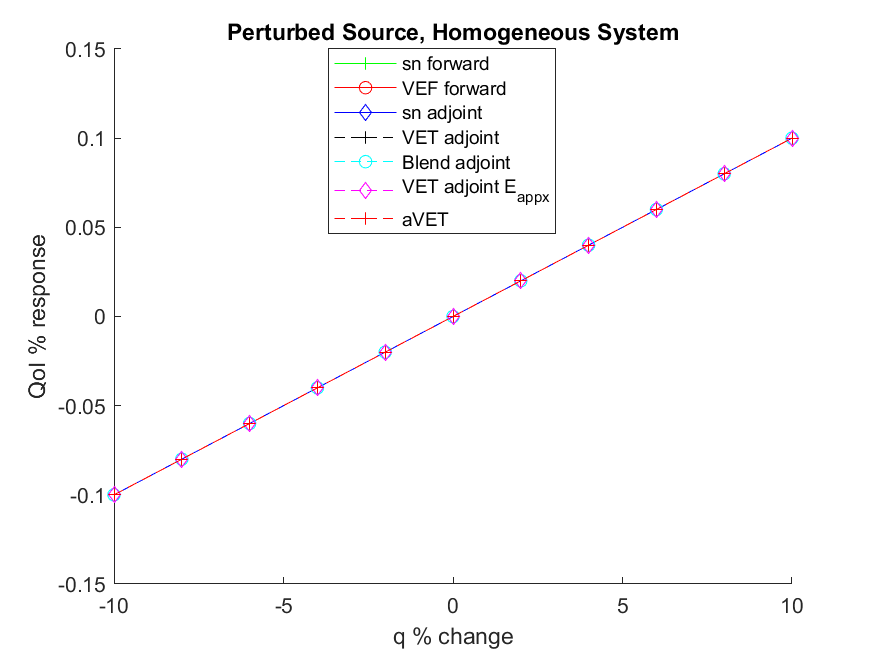
\includegraphics[width=.98\linewidth]{figures2/22qSens.png}
  \label{T1:sfig1}
\end{subfigure}%
\begin{subfigure}{.5\textwidth}
  \centering
  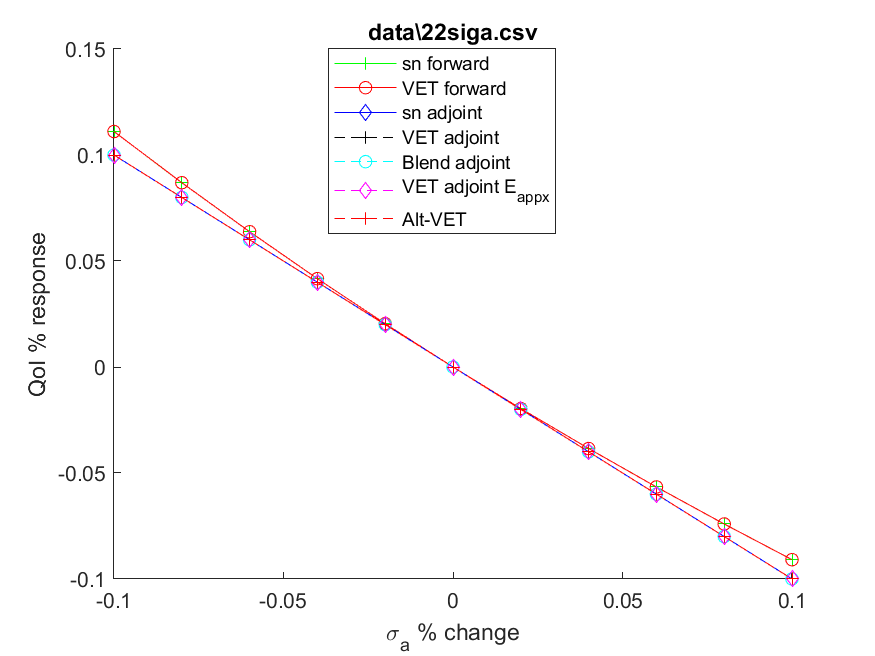
\includegraphics[width=.98\linewidth]{figures2/22sigaSens.png}
  \label{T1:sfig2}
\end{subfigure}
%
\begin{subfigure}{.5\textwidth}
  \centering
  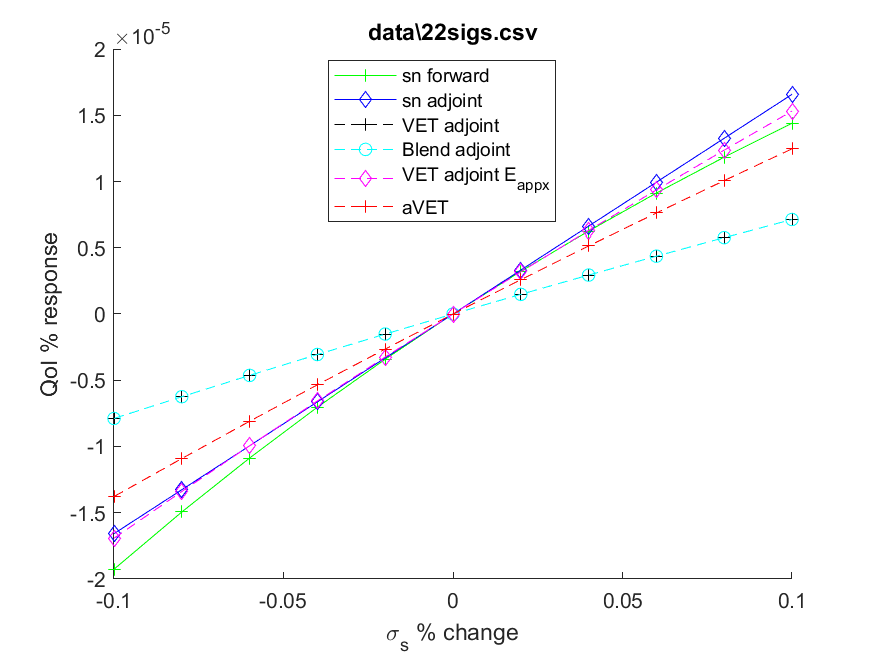
\includegraphics[width=.98\linewidth]{figures2/22sigsSens.png}
  \label{T1:sfig3}
\end{subfigure}%
\begin{subfigure}{.5\textwidth}
  \centering
  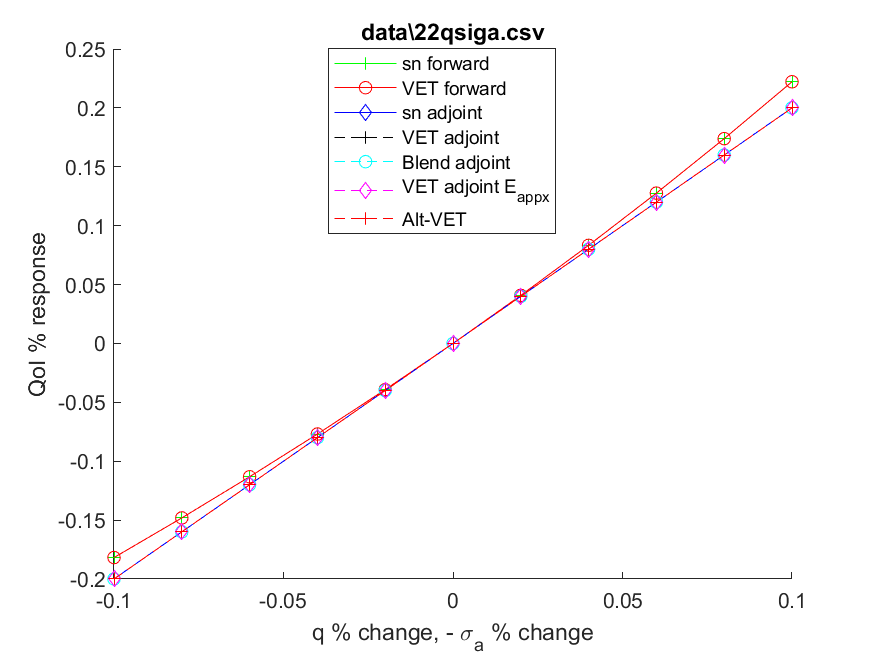
\includegraphics[width=.98\linewidth]{figures2/22qsigaSens.png}
  \label{T1:sfig4}
\end{subfigure}
\caption{\qoi response to various perturbation scenarios for the homogeneous system under various homogeneous perturbations. For the unperturbed system $q=2$, $\sigt=1$, and $\sigs=1$.}
\end{figure}

In both the unperturbed and perturbed state, the Eddington is essentially at the infinite medium limit, so the unperturbed Eddington approximation should be a safe assumption to make in this scenario. The results of the $q$ and $\siga$ perturbations seem to support this. For the source perturbations, no first order approximation is needed, so all methods appear to give the same result. The $\siga$ perturbations begin to show the affects of the first order approximation, adjoint methods diverge from the exact forward methods. As would be expected, the system does not show strong sensitivity to $\sigs$ perturbations.

\begin{table}[H]
\label{TableT1}
\centering
  \begin{tabular}{| l | r || r | r | r | r |}
    \hline
    Method  & $\qoi$ & $+10\% q $  & $-10\% \siga $ & $+10\% \sigs $ & $+10\% q,-10\% \siga$ \\ \hline
     SN Fwd 			&3.99976	&0.39998 &0.44419 &5.7577e-05 & 0.88858\\ \hline
     VET Fwd			&3.99976	&0.39998 &0.44428 &2.7131e-05 &0.88868\\ \hline
     SN Adj			    &3.99976	&0.39998 &0.39983 &6.6307e-05 &0.79980\\ \hline
     VET Adj 			&3.99976	&0.39998 &0.39988 &2.8534e-05 &0.79986\\ \hline
     Blended 			&-			&0.39998 &0.39988 &2.8534e-05 &0.79986\\ \hline
     VET $\delta \Edd$ 	&-			&0.39998 &0.39983 &5.9537e-05 &0.79981\\ \hline
     aVET				&3.99976 	&0.39998 &0.39980  &4.986e-05	 &0.79978\\ \hline
    \end{tabular}
  \caption{Table of selected $\delta \qoi$ values for the homogeneous system under homogeneous perturbations. The unperturbed $\qoi$ for various methods is given in the first column.}
\end{table}


%%%%%%%----------------------------------------------------------------------------------------------
\subsection{Homogeneous System, Inhomogeneous Perturbation}
The initial homogeneous unperturbed system is retained from the previous trial. Now the system is subjected to inhomogeneous perturbations. To accomplish this, only the left $3/5$th of the system experiences the perturbation. This creates generates a material boundary which tends to generate perturbations in $\delta E$.

\begin{figure}[H]
\label{Trial2}
\centering
\begin{subfigure}{.5\textwidth}
  \centering
  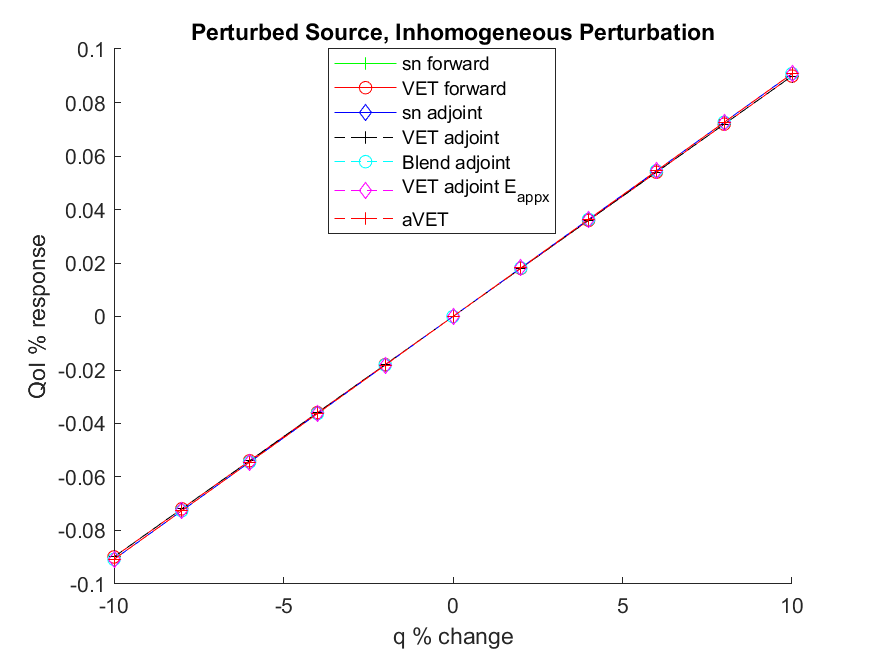
\includegraphics[width=.98\linewidth]{figures2/23qSens.png}
  \label{T2:sfig1}
\end{subfigure}%
\begin{subfigure}{.5\textwidth}
  \centering
  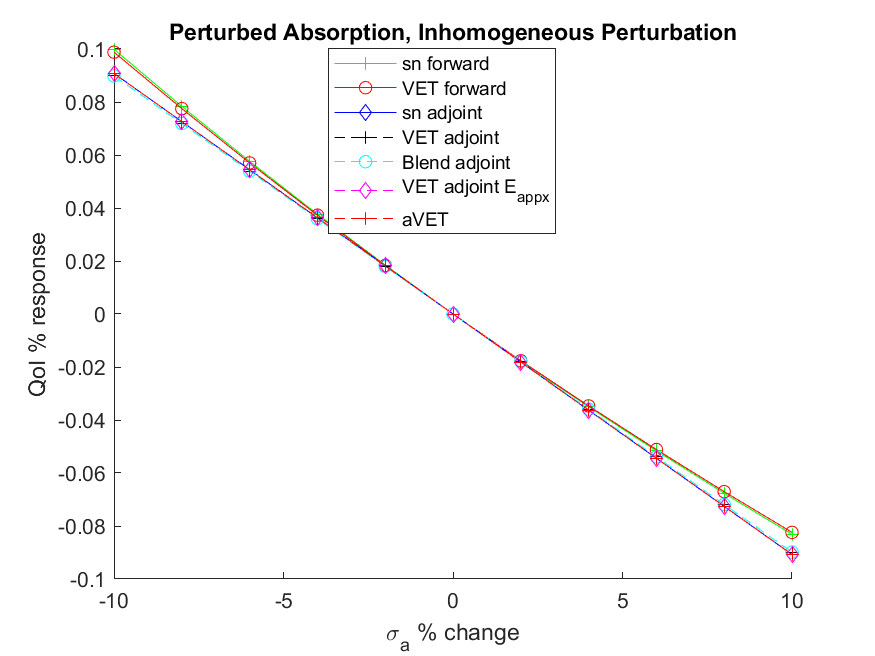
\includegraphics[width=.98\linewidth]{figures2/23sigaSens.png}
  \label{T2:sfig2}
\end{subfigure}
%
\begin{subfigure}{.5\textwidth}
  \centering
  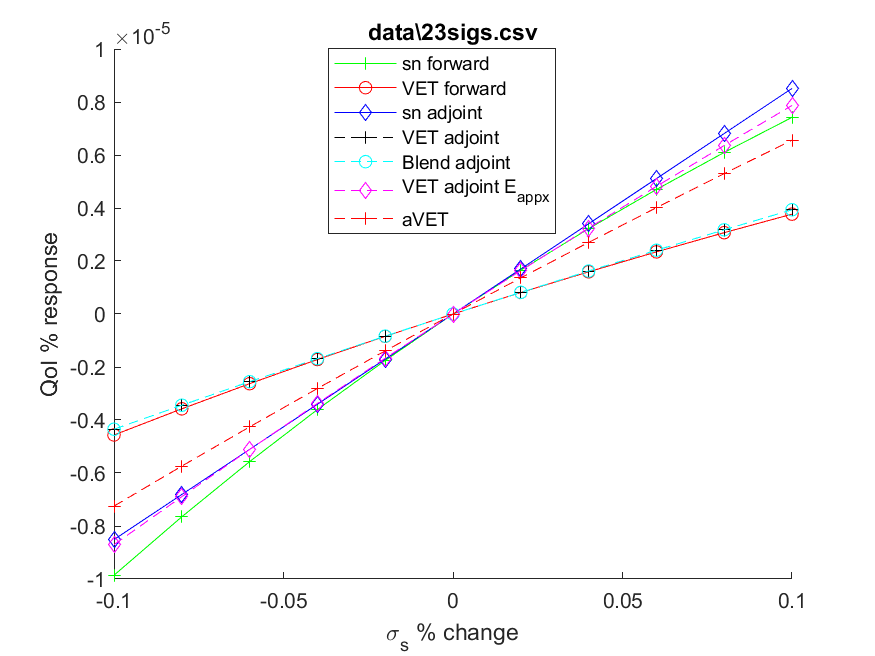
\includegraphics[width=.98\linewidth]{figures2/23sigsSens.png}
  \label{T2:sfig3}
\end{subfigure}%
\begin{subfigure}{.5\textwidth}
  \centering
  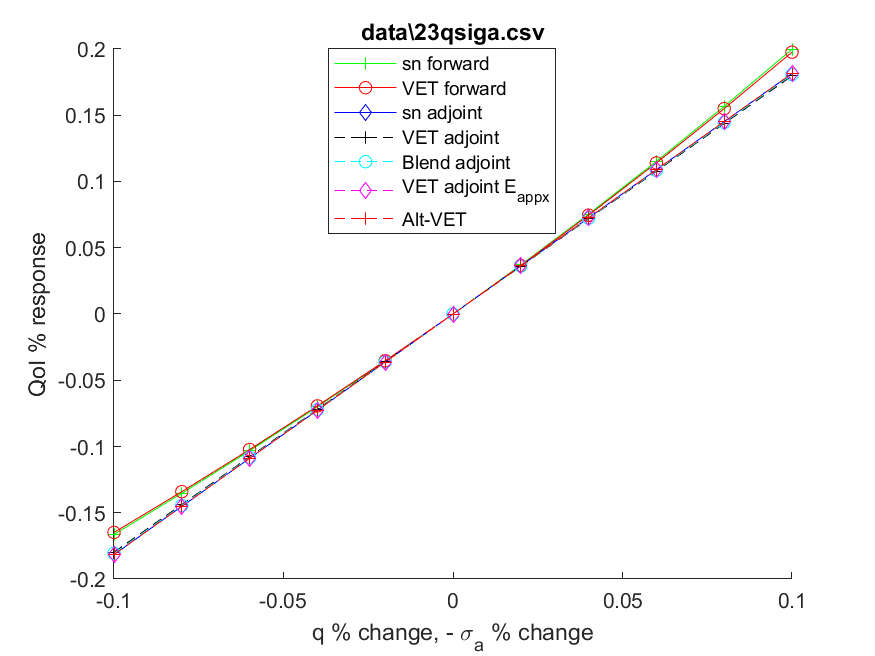
\includegraphics[width=.98\linewidth]{figures2/23qsigaSens.png}
  \label{T2:sfig4}
\end{subfigure}
\caption{\qoi response to various perturbation scenarios for the homogeneous system under various inhomogeneous perturbations. For the unperturbed system $q=2$, $\sigt=1$, and $\sigs=1$.}
\end{figure}

The introduction of the boundary layer in the perturbed state begins to show differentiation in the selected methods. For source perturbations the adjoint methods match their respective forward found values. The blended method matches the SN values for source perturbations and the VET values for cross-section perturbations as designed. The behavior of the blended method with both source and cross-section perturbations shows that it does provide an improvement over the adjoint VET method, however the found value still lies closer to the VET value than the SN adjoint value. The $\delta \Edd$ method shows more promise in this trial, as the addition of the $\delta \Edd$ terms begins to reconcile the VET adjoint method with the more exact SN adjoint. The alternate VET method shows its exact nature for the source perturbation, as well as being the VET method with the closest value to the SN adjoint for $\siga$ perturbations. 


\begin{table}[H]
\centering
  \begin{tabular}{| l | r || r | r | r | r |}
    \hline
    Method  & $\qoi$ & $+10\% q $  & $-10\% \siga $ & $+10\% \sigs $ & $+10\% q,-10\% \siga$ \\ \hline
     SN Fwd 			&3.99976	&0.36309 &0.39952 &2.9680e-05 & 0.79915\\ \hline
     VET Fwd			&3.99976	&0.35947 &0.39517 &1.5072e-05 &0.79040\\ \hline
     SN Adj  			&3.99976	&0.36309 &0.36301 &3.4051e-05 &0.72610\\ \hline
     VET Adj 			&3.99976	&0.35947 &0.35941 &1.5733e-05 &0.71888\\ \hline
     Blended 			&-			&0.36309 &0.35941 &1.5733e-05 &0.72250\\ \hline
     VET $\delta \Edd$ 	&-			&0.36287 &0.36290 &3.0640e-05 &0.72586\\ \hline
     VET Alt			&3.99976	&0.36309 &0.36299 &2.6234e-05 &0.72609\\ \hline
    \end{tabular}
  \caption{Table of selected $\delta \qoi$ values for the homogeneous system under inhomogeneous perturbations. The unperturbed $\qoi$ for various methods is given in the first column.}
\end{table}

%%%%%%%----------------------------------------------------------------------------------------------
\subsection{Shielded Incident Flux}
To observe the response to perturbations in the incident flux, a simple shielding system is tested. Flux is incident on the left side of the system. The incident flux passes though a shield of width 1 with $\siga=0.5$ and $\sigs=0.5$. The response is taken on the right side of the shield.


\begin{figure}[H]
\label{Trial3}
\centering
\begin{subfigure}{.5\textwidth}
  \centering
  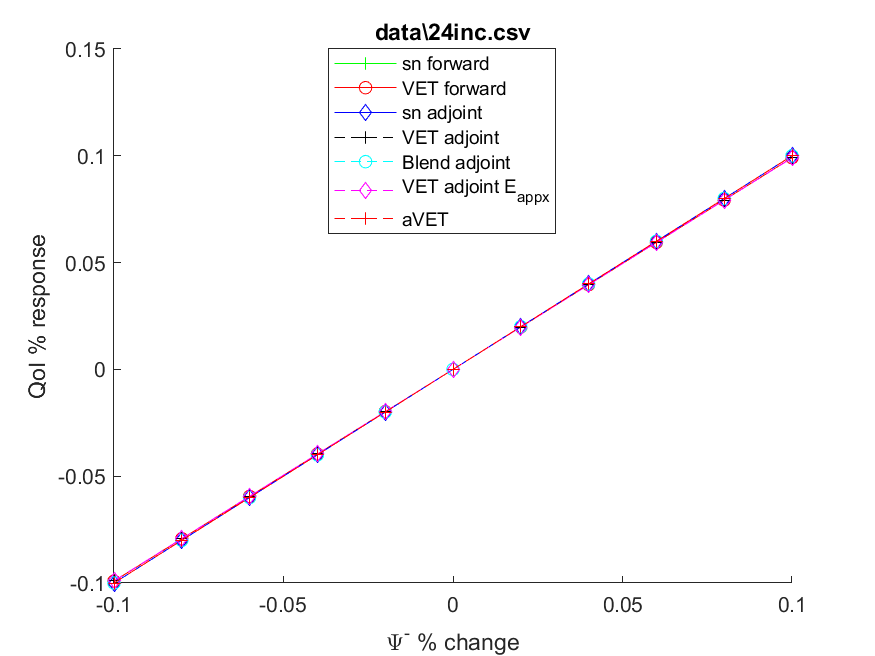
\includegraphics[width=.98\linewidth]{figures2/24incSens.png}
  \label{T3:sfig1}
\end{subfigure}%
\begin{subfigure}{.5\textwidth}
  \centering
  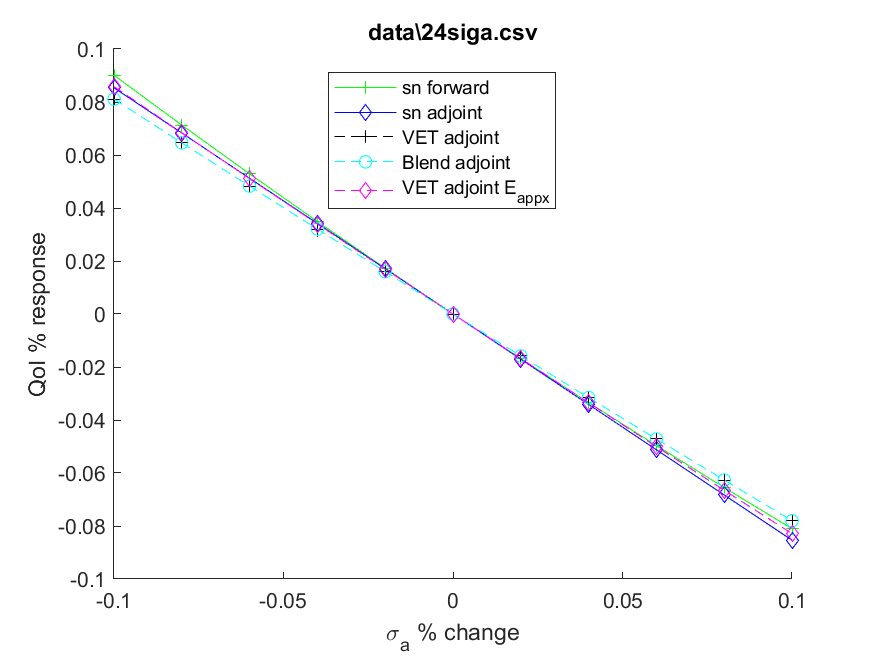
\includegraphics[width=.98\linewidth]{figures2/24sigaSens.png}
  \label{T3:sfig2}
\end{subfigure}
%
\begin{subfigure}{.5\textwidth}
  \centering
  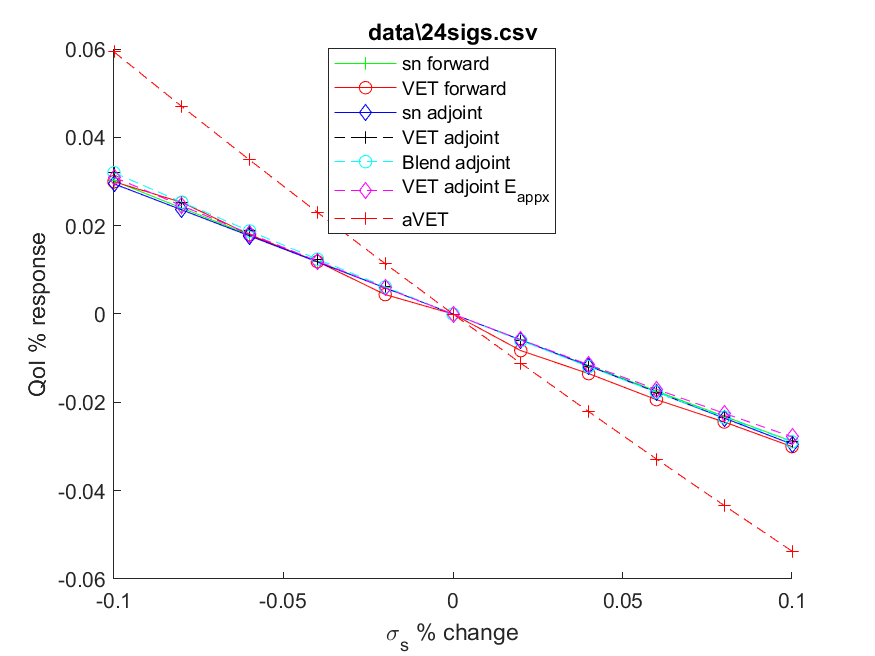
\includegraphics[width=.98\linewidth]{figures2/24sigsSens.png}
  \label{T3:sfig3}
\end{subfigure}%
\begin{subfigure}{.5\textwidth}
  \centering
  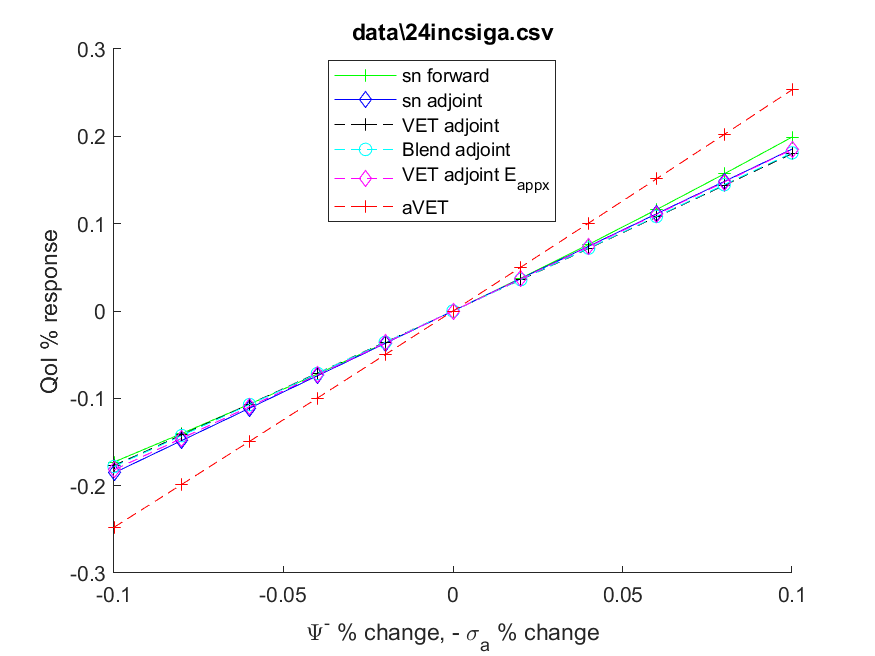
\includegraphics[width=.98\linewidth]{figures2/24incsigaSens.png}
  \label{T3:sfig4}
\end{subfigure}
\caption{\qoi response to various perturbation scenarios for the.}
\end{figure}

Response to perturbation in the incident flux behaves as expected, in that adjoint methods match their respective forward found values. The $\delta E$ approximation method helps approach the SN value in most cases, however when dealing with scattering perturbations, the $\delta E$ method actually results in a $\delta \qoi$ value further from the SN value than the basic VET method. The alternate VET method is as expected exact for the incident flux perturbations, but shows issues with cross-section perturbations in this test case.

\begin{table}[H]
\centering
  \begin{tabular}{| l | r || r | r | r | r |}
    \hline
    Method  & $\qoi$ & $+10\% \psi^- $  & $-10\% \siga $ & $+10\% \sigs $ & $+10\% \psi^-,-10\% \siga$ \\ \hline
     SN Fwd 			&0.234008 	&0.023401 &0.021079 &-0.0067476 & 0.046588\\ \hline
     VET Fwd			&0.234008 	&0.023181 &0.019670 &-0.0066481 &0.044818\\ \hline
     SN Adj  			&0.231931 	&0.023401 &0.019975 &-0.0068956 &0.043376\\ \hline
     VET Adj 			&0.231698 	&0.023181 &0.018981 &-0.0067751 &0.042162\\ \hline
     Blended 			&-			&0.023401 &0.018981 &-0.0067751 &0.042381\\ \hline
     VET $\delta \Edd$ 	&-			&0.023181 &0.020070 &-0.0065156 &0.043251\\ \hline
     VET Alt			&0.234008 	&0.023401 &0.035869 &-0.012563	&0.059270\\ \hline
    \end{tabular}
  \caption{Table of selected $\delta \qoi$ values for the shielding system under perturbations. The unperturbed $\qoi$ for various methods is given in the first column.}
\end{table}

%%%%%%%----------------------------------------------------------------------------------------------
\subsection{Reed Problem}
As a final test, a more varied and complex system is tested. The system is split into 5 regions of unequal length with properties given below. As for perturbations, $\siga$ experiences perturbations in regions 1 and 4, $\sigs$ is perturbed in regions 4 and 5, and $q$ is perturbed in regions 1 and 4. The system has no incident flux.
\begin{equation*}
\begin{split}
&\text{Region 1: } x \in (0,2), \quad \siga=50, \, 			\sigs=0, \, q=50, \, q^\dag=0 \\
&\text{Region 2: } x \in (2,3), \quad \siga=5, \, 			\sigs=0, \, q=0, \, q^\dag=0 \\
&\text{Region 3: } x \in (3,5), \quad \siga \approx 0, \,	\sigs=0, \, q=0, \, q^\dag=0 \\
&\text{Region 4: } x \in (5,6), \quad \siga=0.1, \, 		\sigs=0.9, \, q=1, \, q^\dag=0 \\
&\text{Region 5: } x \in (6,8), \quad \siga=0.1, \, 		\sigs=0.9, \, q=0, \, q^\dag=1 \\
\end{split}
\end{equation*}


\begin{figure}[H]
\label{Trial4}
\centering
\begin{subfigure}{.5\textwidth}
  \centering
  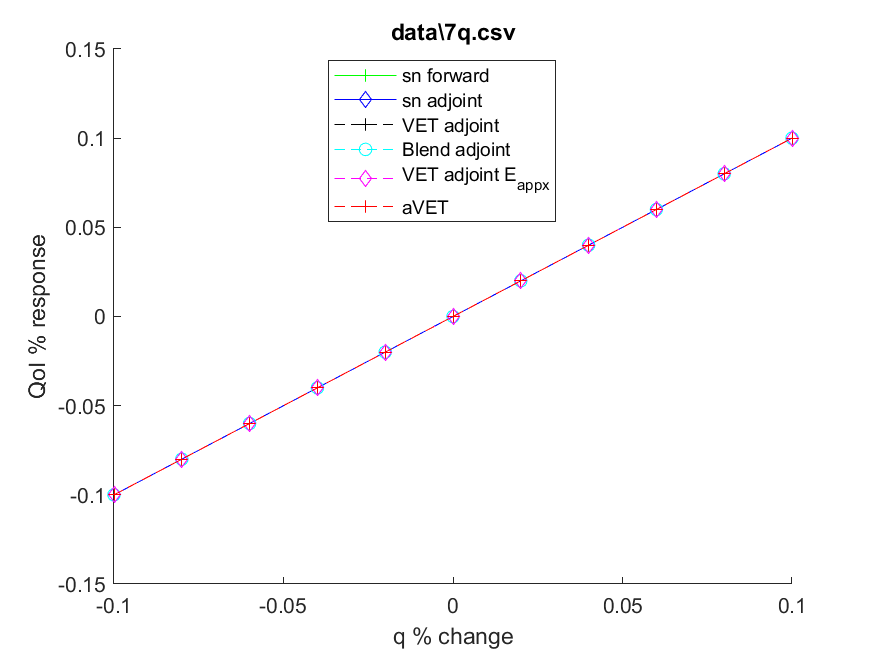
\includegraphics[width=.98\linewidth]{figures2/7qSens.png}
  \label{T4:sfig1}
\end{subfigure}%
\begin{subfigure}{.5\textwidth}
  \centering
  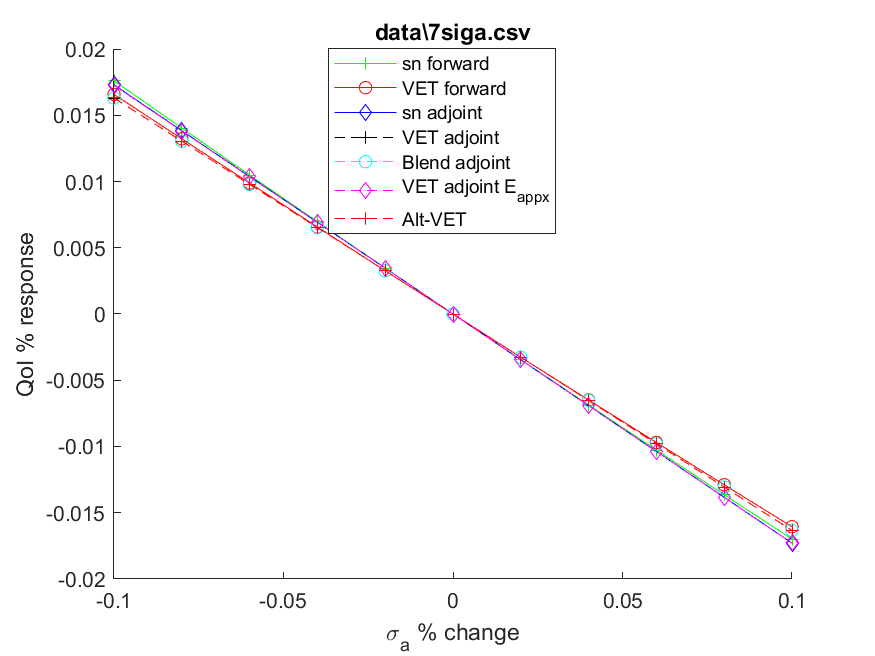
\includegraphics[width=.98\linewidth]{figures2/7sigaSens.png}
  \label{T4:sfig2}
\end{subfigure}
%
\begin{subfigure}{.5\textwidth}
  \centering
  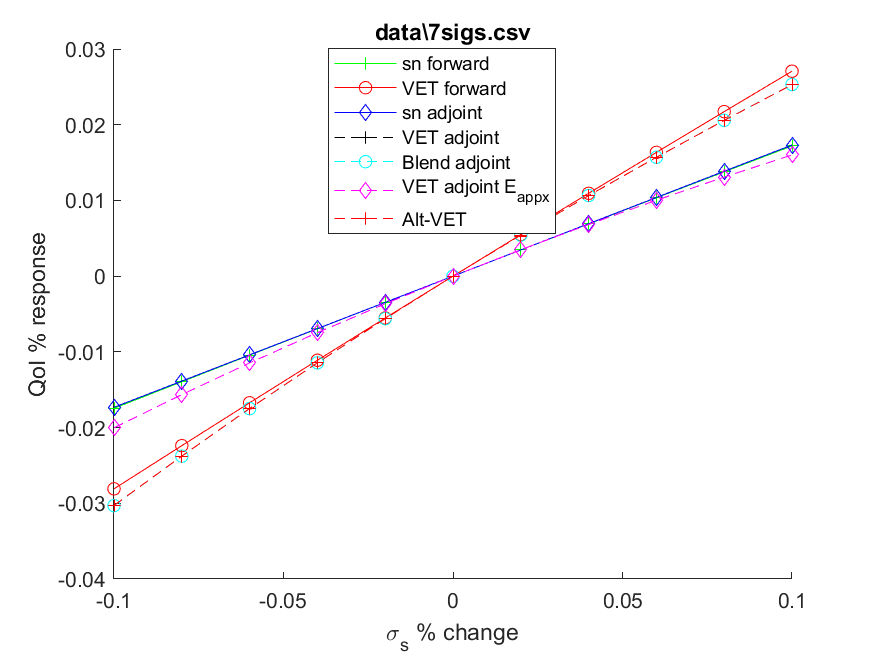
\includegraphics[width=.98\linewidth]{figures2/7sigsSens.png}
  \label{T4:sfig3}
\end{subfigure}%
\begin{subfigure}{.5\textwidth}
  \centering
  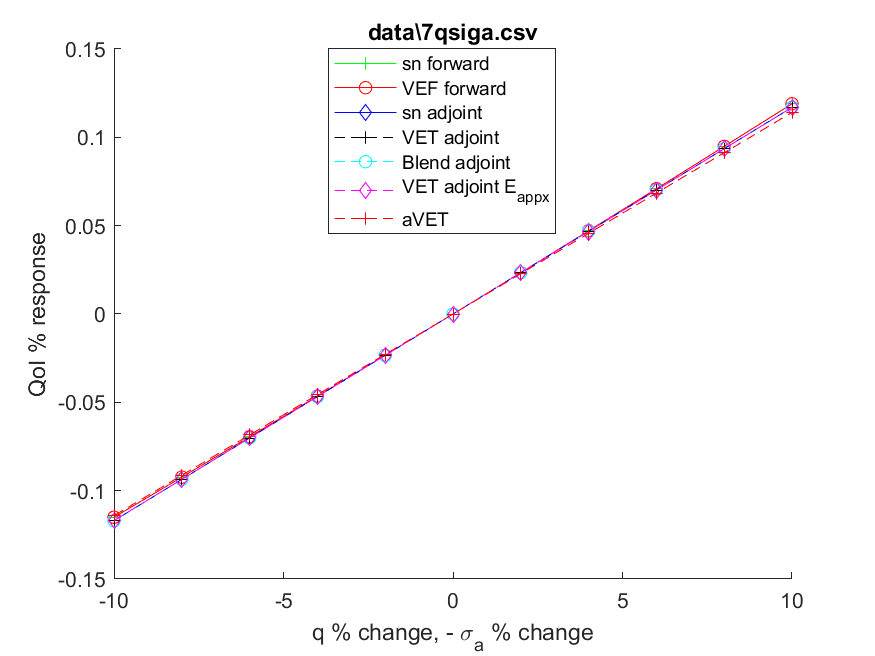
\includegraphics[width=.98\linewidth]{figures2/7qsigaSens.png}
  \label{T4:sfig4}
\end{subfigure}
\caption{\qoi response to various perturbation scenarios for the Reed Problem.}
\end{figure}

The effect of scattering perturbations is more pronounced in the Reed problem, along with the error between the SN and VET derived methods. The $\delta \Edd$ approximation method proves quite valuable in this problem however, and moves the response much closer to the SN adjoint found sensitivity for cross-section perturbations. For cross-section perturbations, the alternate VET method appears closer to VET sensitivity values than SN sensitivity for this test case.

\begin{table}[H]
\centering
  \begin{tabular}{| l | r || r | r | r | r |}
    \hline
    Method  & $\qoi$ & $+10\% q $  & $-10\% \siga $ & $+10\% \sigs $ & $+10\% q,-10\% \siga$ \\ \hline
     SN Fwd 			&1.75802 	&0.17580 &0.030945 &0.030235 & 0.20984\\ \hline
     VET Fwd 			&1.75802 	&0.17561 &0.029105 &0.047568 &0.20763\\ \hline
     SN Adj 			&1.75603  	&0.17580 &0.030401 &0.030450 &0.20620\\ \hline
     VET Adj 			&1.75602  	&0.17561 &0.028580 &0.044778 &0.20419\\ \hline
     Blended 			&-	 		&0.17580 &0.028580 &0.044778 &0.20438\\ \hline
     VET $\delta \Edd$ 	&-		 	&0.17561 &0.030291 &0.028388 &0.20590\\ \hline
     VET Alt		 	&1.75601 	&0.17580 &0.028632 &0.044497 &0.20443\\ \hline
    \end{tabular}
  \caption{Table of selected $\delta \qoi$ values for the Reed system under perturbations. The unperturbed $\qoi$ for various methods is given in the first column.}
\end{table}

\chapter{\uppercase {Conclusion and looking ahead}}

For the systems tested, the VET method shows promise for use in sensitivity calculations. For the majority of the trials the error between the VET and SN adjoint sensitivities was $<10\%$ of the SN sensitivity, and $<1\%$ of the unperturbed QoI. The blended method demonstrated an approach to increase the accuracy, particularly for source perturbations, at the cost of an additional SN solve to obtain $\phi$. The $\delta \Edd$ approximation approach was even more accurate in most cases, but requires at least 1 extra SN solve for each perturbed system property, making it viable in scenarios where many perturbation scenarios must be tested. 

Scattering perturbations showed possibly the most interesting behavior. The deviation of the VET and SN methods is stronger (relative to the SN sensitivity) in most of the test case when $\sigs$ is perturbed. Additionally, the shielding system presented a scenario where the $\delta \Edd$ approach appeared to introduce more error. Unfortunately, the testing of heavy scatting systems in one spacial dimension can be a bit limited. In a two or three dimensions, the ability for particles to scatter around objects exists in general, while this is not present in one dimension. Expanding the discussed concepts to higher spacial dimensions would be a worthwhile next step, particularly in observing the effects of scattering on the VET method.

For the homogeneous test cases, the alternate VET method utilizing $\varphi$ showed obvious advantages by way of it's exact nature for source perturbations and closest values to SN adjoint formulation for $\sigma_a$ perturbations. This method however appeared to have difficulties with the incident flux scenario, returning response values significantly higher than any other method. For the Reed problem, the alternate VET method appeared to return values most similar to the standard VET method, but with the source perturbation response values exact. 

\newpage
\chapter{\uppercase{Appendices}}

\section{APPENDIX A: Time Dependent VET}
While out of scope for this writing, a major goal of this method is the application towards time-dependent systems. As such, it is worth taking a brief look at how the VET formulation would look in a time dependent system. As with the steady state, the starting point is the one-group transport equation, now with the time derivative factor.
\begin{equation}
\label{Trans1GTE}
\frac{1}{v} \frac{\partial}{\partial t} \psi(\vr,\vO,t)+ \vO \cdot \grad \psi(\vr,\vO,t) + \sigt(\vr) \psi(\vr,\vO,t) = \frac{1}{4 \pi} \sigs(\vr) \phi(\vr) + q(\vr,\vO,t), \quad \forall \vr \in V,t \geq 0
\end{equation}
\begin{equation}
\label{Trans1GTE_bc}
\psi(\vr,\vO,t) = \psi^{\text{inc}}(\vr,\vO,t) \quad \vr \in \partial V^{-} = \{ \vr \in \partial V, \text{ s.t. }, \vO \cdot \vec{n}(\vr) < 0\}
\end{equation}
\begin{equation}
\label{Trans1GTE_t0}
\psi(\vr,\vO,0) = \psi_0(\vr,\vO)
\end{equation}
The zero-th and first angular moments are taken of the time dependent system. The Eddington Tensor is used in the 1st order equation.
\begin{subequations}
%
\begin{equation}
\label{0amTrans}
\frac{1}{v} \frac{\partial}{\partial t}\phi + \div \vec{J} + (\siga) \phi = \scalSource \,,
\end{equation}
%
\begin{equation}
\label{1amTrans}
\frac{1}{v} \frac{\partial}{\partial t}\vec{J}  + \div \left( \Edd \phi \right) + \sigt \vec{J} = 0 \,.
\end{equation}
%
\end{subequations}
The moments are then combined in the same fashion used in the steady-state case
\begin{equation}
\label{VETTrans}
\frac{1}{v} \frac{\partial}{\partial t}\phi - \div \left( \frac{1}{v \sigt} \frac{\partial}{\partial t}\vec{J} \right)   - \div \left( \frac{1}{\sigt} \div \left( \Edd \phi \right) \right)  + (\siga) \phi = \scalSource.
\end{equation}
\iwh{Not sure on the exact next step to take. The second term is the ugly one. I can define the residual 
\begin{equation}
f=- \div \left( \frac{1}{\sigt} \div \left( \Edd \phi \right) \right)  + (\siga) \phi - \scalSource
\end{equation}
which is the steady state equation, and muse about how that term must be dealt with accurately to produce time evolution. 
Doing sensitivity we want an operator $A \phi = b$ which the above isn't exactly due to the $\vec{J}$. In addition to $\Edd$ is is reasonable to store some vector value like $\vec{g}=\frac{\vec{J}}{\phi}$? That way there is a well defined $A$ operator to perform the adjoint process on.}

%The next line is the format for inserting new sections.
%Replace the name "newsection"  with the name of your
%new section file.
%\include{data/newsection}


%\bibliography{IanProp} 
%\bibliographystyle{ieeetr}

%fix spacing in bibliography, if any...
%%%%%%%%%%%%%%%%%%%%%%%%%%%%%%%%%%%%%%%%%%%%%%%%%%%%%%%%%%%%%
\let\oldbibitem\bibitem
\renewcommand{\bibitem}{\setlength{\itemsep}{0pt}\oldbibitem}
%%%%%%%%%%%%%%%%%%%%%%%%%%%%%%%%%%%%%%%%%%%%%%%%%%%%%%%%%%%%%%%
%The bibliography style declared is the IEEE format. If
%you require a different style, see the document
%bibstyles.pdf included in this package. This file,
%hosted by the University of Vienna, shows several
%bibliography styles and examples of in-text citation
%and a references page.
\bibliographystyle{ieeetr}

\phantomsection
\addcontentsline{toc}{chapter}{REFERENCES}

\renewcommand{\bibname}{{\normalsize\rm REFERENCES}}

%This file is a .bib database that contains the sources.
%This removes the dependency on the previous file
%bibliography.tex.
\bibliography{QoI_MS}




%This next line includes appendices. The file
%appendix.tex contains commands pointing to
%the appendix files; be sure to change these
%pointers if you end up changing the filenames.
%Leave this commented if you will not need
%appendix material.
%%%%%%%%%%%%%%%%%%%%%%%%%%%%%%%%%%%%%%%%%%%%%%%%%%%%
%
%  New template code for TAMU Theses and Dissertations starting Fall 2016.  
%
%
%  Author: Sean Zachary Roberson
%  Version 3.17.06
%  Last Updated: 6/15/2017
%
%%%%%%%%%%%%%%%%%%%%%%%%%%%%%%%%%%%%%%%%%%%%%%%%%%%

\begin{appendices}
\titleformat{\chapter}{\centering\normalsize}{APPENDIX \thechapter}{0em}{\vskip .5\baselineskip\centering}
\renewcommand{\appendixname}{APPENDIX}

%%%%%%%%%%%%%%%%%%%%%%%%%%%%%%%%%%%%%%%%%%%%%%%%%%%
%
%  New template code for TAMU Theses and Dissertations starting Fall 2016.
%
%
%  Author: Sean Zachary Roberson 
%	 Version 3.16.09
%  Last updated 9/12/2016
%
%%%%%%%%%%%%%%%%%%%%%%%%%%%%%%%%%%%%%%%%%%%%%%%%%%%

%%%%%%%%%%%%%%%%%%%%%%%%%%%%%%%%%%%%%%%%%%%%%%%%%%%%%%%%%%%%%%%%%%%%%%
%%                           APPENDIX A 
%%%%%%%%%%%%%%%%%%%%%%%%%%%%%%%%%%%%%%%%%%%%%%%%%%%%%%%%%%%%%%%%%%%%%

\phantomsection

\chapter{\uppercase{First Appendix}}

Text for the Appendix follows.

\begin{figure}[h]
\centering
%\includegraphics[scale=.50]{figures/Penguins.jpg}
\caption{TAMU figure}
\label{fig:tamu-fig5}
\end{figure}

%%%%%%%%%%%%%%%%%%%%%%%%%%%%%%%%%%%%%%%%%%%%%%%%%%%
%
%  New template code for TAMU Theses and Dissertations starting Fall 2016.
%
%
%  Author: Sean Zachary Roberson 
%	 Version 3.16.09 
%  Last updated 9/12/2016
%
%%%%%%%%%%%%%%%%%%%%%%%%%%%%%%%%%%%%%%%%%%%%%%%%%%%

%%%%%%%%%%%%%%%%%%%%%%%%%%%%%%%%%%%%%%%%%%%%%%%%%%%%%%%%%%%%%%%%%%%%%%
%%                           APPENDIX B
%%%%%%%%%%%%%%%%%%%%%%%%%%%%%%%%%%%%%%%%%%%%%%%%%%%%%%%%%%%%%%%%%%%%%

\chapter{\uppercase {A Second Appendix Whose Title Is Much Longer Than The First}}

Text for the Appendix follows.

\begin{figure}[h]
\centering
%\includegraphics[scale=.50]{figures/Penguins.jpg}
\caption{Another TAMU figure.}
\label{fig:tamu-fig6}
\end{figure}

\section{Appendix Section}

\section{Second Appendix Section}


\pagebreak{}

\end{appendices}


\end{document}
